\documentclass[10pt]{article}
\usepackage[utf8]{inputenc}
\usepackage[T1]{fontenc}
\usepackage{amsmath}
\usepackage{amsfonts}
\usepackage{amssymb}
\usepackage[version=4]{mhchem}
\usepackage{stmaryrd}
\usepackage{bbold}
\usepackage{graphicx}
\usepackage[export]{adjustbox}
\graphicspath{ {./images/} }
\usepackage{caption}
\usepackage{hyperref}
\hypersetup{colorlinks=true, linkcolor=blue, filecolor=magenta, urlcolor=cyan,}
\urlstyle{same}
\usepackage{multirow}

\title{Pushing the QAM method for finding APN functions further }

\author{Nadiia Ichanska ${ }^{1}$, Simon Berg ${ }^{1}$, Nikolay S. Kaleyski ${ }^{1}$, Yuyin Yu ${ }^{2}$\\
${ }^{1}$ University of Bergen, Norway\\
${ }^{2}$ School of Mathematics and Information Science, Guangzhou University, China}
\date{}


%New command to display footnote whose markers will always be hidden
\let\svthefootnote\thefootnote
\newcommand\blfootnotetext[1]{%
  \let\thefootnote\relax\footnote{#1}%
  \addtocounter{footnote}{-1}%
  \let\thefootnote\svthefootnote%
}

%Overriding the \footnotetext command to hide the marker if its value is `0`
\let\svfootnotetext\footnotetext
\renewcommand\footnotetext[2][?]{%
  \if\relax#1\relax%
    \ifnum\value{footnote}=0\blfootnotetext{#2}\else\svfootnotetext{#2}\fi%
  \else%
    \if?#1\ifnum\value{footnote}=0\blfootnotetext{#2}\else\svfootnotetext{#2}\fi%
    \else\svfootnotetext[#1]{#2}\fi%
  \fi
}

\begin{document}
\maketitle
\captionsetup{singlelinecheck=false}


\begin{abstract}
APN functions offer optimal resistance to differential attacks and are instrumental in the design of block ciphers in cryptography. While finding APN functions is very difficult in general, a promising way to construct APN functions is through symmetric matrices called Quadratic APN matrices (QAM). It is known that the search space for the QAM method can be reduced by means of orbit partitions induced by linear equivalences. This paper builds upon and improves these approaches in the case of homogeneous quadratic functions over $\mathbb{F}_{2^{n}}$ with coefficients in the subfield $\mathbb{F}_{2^{m}}$. We propose an innovative approach for computing orbit partitions for cases where it is infeasible due to the large search space, resulting in the applications for the dimensions $(n, m)=(8,4)$, and $(n, m)=(9,3)$. We find and classify, up to CCZ-equivalence, all quadratic APN functions for the cases of $(n, m)=(8,2)$, and $(n, m)=(10,1)$, discovering a new APN function in dimension 8. Also, we show that an exhaustive search for $(n, m)=(10,2)$ is infeasible for the QAM method using currently available means, following partial searches for this case.
\end{abstract}

\section*{1 Introduction}
Cryptographically optimal classes of functions such as almost perfect nonlinear (APN) functions play a crucial role in cryptography, particularly in designing secure symmetric ciphers. S-boxes or substitution boxes together with their properties characterize the security of the cipher. They are fundamental building blocks, and therefore, they must withstand various attacks, such as linear and differential cryptanalysis. The effectiveness of an S-box in thwarting these attacks largely depends on certain mathematical properties, with differential uniformity being one of the most important since it measures the resistance to differential cryptanalysis, one of the most efficient attacks that can be applied against block ciphers. The lower the differential uniformity of a function, the more resistant it is to differential attacks. An APN function is an optimal type of S-box function with the lowest differential uniformity possible. These functions achieve therefore maximal security against differential attacks, making them highly desirable in cryptography. Since at the same time, they are mathematically rare and challenging to identify, discovering new APN functions often requires extensive computation and sophisticated methods. These methods span a wide range, from theoretical approaches to brute-force and heuristic computational searches. One example of the recent innovations in computational searches is the QAM Method [15], which involves a depth-first search through symmetric matrices representing the S-box.

This paper explores and advances the Quadratic APN Matrix (QAM) method for searching for Almost Perfect Nonlinear (APN) functions. Originally introduced in 2014 by Y. Yu, M. Wang,

\footnotetext{This paper was presented in part under the title "Further Investigations on the QAM Method for Finding APN Functions" at the 9th International Workshop on Boolean Functions and their Applications (BFA 2024). Sections 3.3; 3.5; 4.1; 4.5.1; 5.1; 5.4.2 are new.
}
and Y. Li [15], the QAM method was used to discover 2252 APN functions; this count was later increased to 8157 in the extended version [14]. In 2020, this approach was used to classify all quadratic APN functions over the finite field $\mathbb{F}_{2^{n}}$ with coefficients in the prime field $\mathbb{F}_{2}$ up to dimension $n=9$ [11], which was recently pushed forward to dimension 10 in [12]. Later, in 2022, D. Davidova and N.S. Kaleyski [7] expanded on this by considering subfields other than prime fields and proposing a more intuitive definition of the derivative matrix.

In this work, we introduce an improved computational framework for applying the QAM method to search for quadratic APN functions with subfield coefficients. We use linear permutations to reduce the search space beyond the first level of the depth-first search (as opposed to all other previous papers, where such a reduction is only applied to the first level) and introduce an approach to test if two values belong to the same orbit under the action of linear permutations, allowing the method to be used in the case of higher dimensions where generating all linear permutations explicitly is infeasible. We also describe an approach for estimating the running time by representing the search as a tree. This also allows us to efficiently distribute parallel processes during the search. Additionally, we enhance the computational speed by applying linear equivalence on the right and improve upon the submatrix test from [15], which can be used to prune away branches of the search that do not lead to APN functions. By generalizing the result from [12] we also refine the QAM test.

This allows us to conduct a full classification of quadratic APN functions over $\mathbb{F}_{2^{n}}$ with coefficients in $\mathbb{F}_{2^{m}}$ in the cases of $(n, m)=(10,1)$ and $(n, m)=(8,2)$. In the case of ( 10,1 ), we confirm that all of these functions belong to the previously known classes, while in the case of $(8,2)$ we find one new APN function, which is inequivalent to all the previously known ones.

\section*{2 Preliminaries}
Consider $n, m$ natural numbers. We use $\mathbb{F}_{2}^{n}$ to represent the vector space of dimension $n$ over the finite field $\mathbb{F}_{2}$ with 2 elements. A function $F$ that maps from $\mathbb{F}_{2}^{n}$ to $\mathbb{F}_{2}^{m}$ is referred to as an (n,m)-function, a vectorial Boolean function, or S-box.

The algebraic normal form (ANF) of an ( $n, m$ )-function $F$ is the unique representation:

$$
F\left(x_{1}, x_{2}, \ldots, x_{n}\right)=\sum_{u \in \mathbb{F}_{p^{n}}} a_{u} \cdot \prod_{i=1}^{n} x_{i}^{u_{i}}, a_{u} \in \mathbb{F}_{2}^{m}
$$

where $x=\left(x_{1}, x_{2}, \ldots, x_{n}\right)$ and $u=\left(u_{1}, u_{2}, \ldots, u_{n}\right)$ are the coordinate vectors of $x$ and $u$, respectively. The algebraic degree of an $(n, m)$-function $F$ is defined as the highest degree of any term with a non-zero coefficient in ANF representation, that is $\operatorname{deg}(F)=\max \left\{\sum_{i=1}^{n} u_{i} \mid a_{u} \neq 0, u=\right. \left.\left(u_{1}, u_{2}, \ldots, u_{n}\right) \in \mathbb{F}_{2}^{n}\right\}$. A function $F$ with an algebraic degree not exceeding 1 is called affine, or equivalently it satisfies $F(x)+F(y)+F(z)=F(x+y+z)$ for any $x, y, z$ in $\mathbb{F}_{2^{n}}$. If for an affine $F$ we also have $F(0)=0$, we say that $F$ is linear. Functions with algebraic degrees of 2 and 3 are referred to as quadratic and cubic, respectively.

The finite field $\mathbb{F}_{2^{n}}$ has the structure of $n$-dimensional vector space, by choosing $\mathbb{F}_{2}$-basis $\left(\alpha_{1}, \ldots, \alpha_{n}\right)$ of $\mathbb{F}_{2^{n}}$, every element $v \in \mathbb{F}_{2}^{n}$ can be identified with $v_{1} \alpha_{1}+\cdots+\alpha_{n} v_{n}$. Therefore vector space $\mathbb{F}_{2}^{n}$ can be identified with the finite field $\mathbb{F}_{2^{n}}$. For an $(n, m)$-function $F$ where $m$ divides $n$, it can be represented as a polynomial over $\mathbb{F}_{2^{n}}$ of the form $F(x)=\sum_{i=0}^{2^{n}-1} a_{i} \cdot x^{i}, a_{i} \in \mathbb{F}_{2^{n}}$. This is called the univariate representation of $F$. This representation always exists, and when $n=m$, this representation is unique.

For any $(n, m)$-function $F: \mathbb{F}_{2^{n}} \rightarrow \mathbb{F}_{2^{m}}$, its (first-order) derivative in the direction $a \in \mathbb{F}_{2^{n}} \backslash\{0\}$ is $D_{a} F(x)=F(a+x)+F(x)$. The differential uniformity $\delta_{F}$ of an $(n, m)$-function $F$ is the\\
maximum number of solutions $x$ to any equation of the form $F(a+x)+F(x)=b$ for any choice of $a, b$ in $\mathbb{F}_{2^{n}}$ with $a \neq 0$, or symbolically:

$$
\delta_{F}=\max _{a, b \in \mathbb{F}_{2^{n}, a \neq 0}}\left|\left\{x \in \mathbb{F}_{2^{n}}: D_{a} F(x)=b\right\}\right|
$$

Differential uniformity measures the resistance of a function to a differential attack. The smaller $\delta_{F}$ - the better its resistance. For the case of characteristic 2 , the smallest differential uniformity that can be achieved is $\delta_{F}=2$. The functions $F: \mathbb{F}_{2^{n}} \rightarrow \mathbb{F}_{2^{m}}$ with $\delta_{F}=2$ are called almost perfect nonlinear (APN) and have the best possible resistance to differential attacks. We design a computational approach based on the method of symmetric matrices [15], [7] to find and classify all APN functions for particular dimensions with coefficients in subfields.

There are several equivalence relations of functions for which differential uniformity is an invariant. Consequently, having a single APN function allows us to generate an extensive class of equivalent APN functions. Therefore, APN functions are typically considered up to equivalence, allowing us to prune equivalent functions during an exhaustive search once a representative from each equivalent class is identified. Two functions $F$ and $F^{\prime}$ from $\mathbb{F}_{2}^{n}$ to $\mathbb{F}_{2}^{m}$ are called affine equivalent (or linear equivalent) if there exist affine (linear) permutations $A_{1}$ of $\mathbb{F}_{2}^{m}$ and $A_{2}$ of $\mathbb{F}_{2}^{n}$ s.t. $F^{\prime}=A_{1} \circ F \circ A_{2}$. Moreover, we say that $F$ and $F^{\prime}$ from $\mathbb{F}_{2}^{n}$ to $\mathbb{F}_{2}^{m}$ are extended affine equivalent(EA-equivalent) if there exists an affine mapping $A: \mathbb{F}_{2}^{n} \rightarrow \mathbb{F}_{2}^{m}$ and affine permutations $A_{1}$ of $\mathbb{F}_{2}^{m}$ and $A_{2}$ of $\mathbb{F}_{2}^{n}$ s.t. $F^{\prime}=A_{1} \circ F \circ A_{2}+A$. The most general known equivalence relation that is used in practice and preserves the differential uniformity is called CCZ-equivalence. Two functions $F$ and $F^{\prime}$ from $\mathbb{F}_{2}^{n}$ to $\mathbb{F}_{2}^{m}$ are called Carlet-Charpin-Zinoviev equivalent (CCZ-equivalent) if there exists an affine permutation $A$ of $\mathbb{F}_{2}^{n} \times \mathbb{F}_{2}^{m}$ that maps the image of the graph of $F$ to the graph of $F^{\prime}$, i.e. $A\left(G_{F}\right)=G_{F^{\prime}}$, where $G_{F}=\left\{(x, F(x)) \mid x \in \mathbb{F}_{2}^{n}\right\}$ and $G_{F^{\prime}}=\left\{\left(x, F^{\prime}(x)\right) \mid x \in \mathbb{F}_{2}^{n}\right\}$. In the literature, APN functions are typically classified up to CCZequivalence. We also use the differential spectrum that serves as an invariant that can distinguish between inequivalent APN functions. The differential spectrum $\mathcal{D}_{F}$ of the function $F$ is the multiset of all values $\delta_{F}(a, b)$ for each pair $(a, b)$ where $a \neq 0$, i.e. $\mathcal{D}_{F}=\left[\delta_{F}(a, b): a, b \in \mathbb{F}_{2^{n}}, a \neq 0\right]$, where $\delta_{F}(a, b)$ is the number of solutions in $x$ to the equation $D_{a} F(x)=b$.

This multiset $\mathcal{D}_{F}$ represents the distribution of all the values ( $a, b$ ) across all non-zero input differences $a$ and output differences $b$. The ortho-derivative [5] of a quadratic function $F: \mathbb{F}_{2}^{n} \mapsto \mathbb{F}_{2}^{n}$ is a function $\pi: \mathbb{F}_{2}^{n} \mapsto \mathbb{F}_{2}^{n}$, s.t. $\pi(0)=0$, and for all $x, a \in \mathbb{F}_{2}^{n}, a \neq 0$ we have $\pi(a) \neq 0$ and:

$$
\pi(a) \cdot(F(x)+F(x+a)+F(0)+F(a))=0
$$

We refer to the [6] as a general reference to APN functions and their cryptographic properties.

Unless explicitly stated otherwise, we assume henceforth that we are dealing with $F: \mathbb{F}_{2^{n}} \rightarrow \mathbb{F}_{2^{n}}$ functions with identical domain and co-domain. Moreover, we consider quadratic $(n, n)$-functions without linear and affine terms of the form


\begin{equation*}
F(x)=\sum_{0 \leq i<j \leq n-1} a_{i, j} x^{2^{i}+2^{j}}, a_{i, j} \in \mathbb{F}_{2^{n}} . \tag{1}
\end{equation*}


Quadratic functions $F(x)$ with $i \neq j$ are often called purely quadratic or homogeneous quadratic functions. We can omit linear and affine terms due to equivalence. For quadratic $\mathrm{APN}(n, n)$ functions, $F$ and $F^{\prime}$ are CCZ-equivalent if and only if they are EA-equivalent [10].

Let $\mathcal{B}=\left\{b_{1}, b_{2}, \ldots, b_{n}\right\}$ be a basis of a vector space $\mathbb{F}_{2}^{n}$ over a prime field $\mathbb{F}_{2}$. For a coordinate vector $v=\left(v_{1}, \ldots, v_{n}\right) \in \mathbb{F}_{2}^{n}$, we call the rank of the $v$ the dimension of the $\mathbb{F}_{2}$-linear span of\\
its coordinates over $\mathbb{F}_{2}$. Let $\mathbb{F}_{2^{n}}^{m \times k}$ denote the space of all matrices over $\mathbb{F}_{2^{n}}$ with $m$ rows and $k$ columns. We will use the notation $M_{i, j}$ to refer to the entry in the $i$-th row and $j$-th column of the matrix $M \in \mathbb{F}_{2^{n}}^{m \times k}, 1 \leq i \leq m, 1 \leq j \leq k$.

The symmetric derivative of a function $F: \mathbb{F}_{2^{n}} \rightarrow \mathbb{F}_{2^{n}}$ in the direction $a \in \mathbb{F}_{2^{n}}$ is


\begin{equation*}
\Delta_{a} F(x)=F(a+x)+F(x)+F(a)+F(0)=D_{a} F(x)+D_{a} F(0) . \tag{2}
\end{equation*}


In [15] the notion of the quadratic APN matrix was introduced together with its properties, while the interpretation of this structure as a matrix of symmetric derivatives was given in [7].

The derivative matrix [7],[15] of the function $F$ is the matrix $M_{F} \in \mathbb{F}_{2^{n}}^{n \times n}$ given by

\[
M_{F}=\left[\begin{array}{cccc}
\Delta F\left(b_{1}, b_{1}\right) & \Delta F\left(b_{1}, b_{2}\right) & \ldots & \Delta F\left(b_{1}, b_{n}\right)  \tag{3}\\
\Delta F\left(b_{1}, b_{2}\right) & \Delta F\left(b_{2}, b_{2}\right) & \ldots & \Delta F\left(b_{2}, b_{n}\right) \\
\vdots & \vdots & \ddots & \vdots \\
\Delta F\left(b_{1}, b_{n}\right) & \Delta F\left(b_{2}, b_{n}\right) & \ldots & \Delta F\left(b_{n}, b_{n}\right)
\end{array}\right]
\]

where we denote $\Delta_{b_{i}} F\left(b_{j}\right)$ as $\Delta F\left(b_{i}, b_{j}\right)$, because $\Delta_{b_{i}} F\left(b_{j}\right)=\Delta_{b_{j}} F\left(b_{i}\right)$, for any $1 \leq i, j \leq n$. A matrix $M_{F} \in \mathbb{F}_{2^{n}}^{n \times n}$ is called a Quadratic APN Matrix (QAM) [15] if:

\begin{enumerate}
  \item $M_{F}$ is symmetric and the elements in its main diagonal are all zeros;
  \item Every nonzero linear combination of the $n$ rows (or columns, since $M_{F}$ is symmetric) of $M_{F}$ has rank $n-1$.
\end{enumerate}

Following the Corollary 5 from [7], we get that a function (1) is APN if and only if its derivative matrix $M_{F}$ is QAM. This allows us to conduct a depth-first search for all quadratic APN functions by traversing all possible derivative matrices.

\section*{3 Improving the QAM method}
Let $n, m$ be natural numbers such that $m$ divides $n$. Set a normal basis $\mathcal{B}=\left\{b, b^{2}, \ldots, b^{2^{n-1}}\right\}$ of $\mathbb{F}_{2^{n}}$ over $\mathbb{F}_{2}$, where $b$ is a normal element. We consider a homogeneous quadratic function over $\mathbb{F}_{2^{n}}$ with coefficients in the subfield $\mathbb{F}_{2^{m}}$ :


\begin{equation*}
F(x)=\sum_{0 \leq i<j \leq n-1} a_{i, j} x^{2^{i}+2^{j}}, \text { for } a_{i, j} \in \mathbb{F}_{2^{m}} \tag{4}
\end{equation*}


The derivative matrix (3) of the function $F(x)$ will look like

\[
M_{F}(\mathcal{B})=\left(\begin{array}{cccc}
\Delta F(b, b) & \Delta F\left(b, b^{2}\right) & \ldots & \Delta F\left(b, b^{2^{n-1}}\right)  \tag{5}\\
\Delta F\left(b^{2}, b\right) & \Delta F\left(b^{2}, b^{2}\right) & \ldots & \Delta F\left(b^{2}, b^{2^{n-1}}\right) \\
\vdots & \vdots & \ddots & \vdots \\
\Delta F\left(b^{2^{n-1}}, b\right) & \Delta F\left(b^{2^{n-1}}, b^{2}\right) & \ldots & \left.\Delta F\left(b^{2^{n-1}}, b^{2^{n-1}}\right)\right)
\end{array}\right)
\]

Using the univariate representation of $F(x)$, it is not so hard to show that

$$
F(x)^{2^{m}}=\left(\sum_{0 \leq i<j \leq n-1} a_{i, j} x^{2^{i}+2^{j}}\right)^{2^{m}}=\sum_{0 \leq i<j \leq n-1} a_{i, j}\left(x^{2^{i}+2^{j}}\right)^{2^{m}}=F\left(x^{2^{m}}\right) .
$$

Applying the same to the symmetric derivative $\Delta_{a} F(x)$ :

$$
\begin{aligned}
\left(\Delta_{a} F(x)\right)^{2^{m}}=(F(x+a)+F(x)+F(a) & +F(0))^{2^{m}}=F(x+a)^{2^{m}}+F(x)^{2^{m}}+F(a)^{2^{m}}+0^{2^{m}}= \\
& =F\left(x^{2^{m}}+a^{2^{m}}\right)+F\left(x^{2^{m}}\right)+F\left(a^{2^{m}}\right)=\Delta_{a^{2^{m}}} F\left(x^{2^{m}}\right)
\end{aligned}
$$

That leads us to the main equation that helps simplify the general structure of the derivative matrix for the function with subfield coefficients, which we will call the diagonalization property:


\begin{equation*}
M_{i+m, j+m}=\left(M_{i, j}\right)^{2^{m}} \tag{6}
\end{equation*}


for $1 \leq i, j \leq n$. When entry index $i+m$ or $j+m$ exceeds $n$, we take $i+m \bmod n$, or $j+m \bmod n$, respectively. The diagonalization property allows us to infer matrix values along diagonals from fixed entries in the matrix $M_{F}(5)$. This significantly reduces the degrees of freedom and therefore the number of levels in a computational search.

\subsection*{3.1 Orbit restrictions}
Following Theorem 3 in [15], if we take any linear permutation $l$ of $\mathbb{F}_{2^{n}}$ and $M \in \mathbb{F}_{2}^{n \times n}$ such that $M$ is QAM of some quadratic APN function $F: \mathbb{F}_{2^{n}} \rightarrow \mathbb{F}_{2^{n}}$, then any matrix $M^{\prime}$ produced by


\begin{equation*}
M_{i, j}^{\prime}=l\left(M_{i, j}\right) \text { for all } 1 \leq i, j \leq n \tag{7}
\end{equation*}


will be the quadratic APN matrix of another function $F^{\prime}=l \circ F$ that is linearly equivalent to $F$, therefore EA-equivalent to $F$.

In the case when we want to take only the coefficients from the subfield $\mathbb{F}_{2^{m}}$ of the quadratic function $F$, we need to take only those linear permutation polynomials $l$ that have the coefficients in $\mathbb{F}_{2^{m}}$ as well, so the diagonalization property (6) is preserved for $M^{\prime}$.

Let us take the univariate representation of the linear permutation polynomial $l=\sum_{i=1}^{n} \alpha_{i} x^{2^{i-1}}$ on $\mathbb{F}_{2^{n}}$ with $\alpha_{i} \in \mathbb{F}_{2^{m}}$. The set $\mathcal{L}$ of all linear ( $n, n$ )-permutations with coefficients in the subfield $\mathbb{F}_{2^{m}}$ forms a group under composition acting on $\mathbb{F}_{2^{n}}$. Then the orbit of $a \in \mathbb{F}_{2^{n}}$ under the action of the group $\mathcal{L}$ can be defined as

$$
\operatorname{Orb}(a, \mathcal{L})=\{l(a): l \in \mathcal{L}\}
$$

We will use the orbit notion to restrict the search space. For any purely quadratic function $F(x)$ with coefficients in the subfield $\mathbb{F}_{2^{m}}$ of the form (4), we can represent its derivative matrix $M_{F} \in \mathbb{F}_{2}^{n \times n}$ as a matrix of the form (using diagonalization property (6)):

\[
M_{F}=\left(\begin{array}{cccccc}
0 & \Omega_{1} & \Omega_{2} & \ldots & \ldots & \ldots  \tag{8}\\
\Omega_{1} & 0 & \ddots & \ddots & \ldots & \ldots \\
\Omega_{2} & \ldots & 0 & \Omega_{1}^{2^{m}} & \Omega_{2}^{2^{m}} & \ldots \\
\vdots & \vdots & \Omega_{1}^{2^{m}} & 0 & \ldots & \ldots \\
\vdots & \vdots & \Omega_{2}^{2^{m}} & \ldots & 0 & \ldots \\
\vdots & \vdots & \vdots & \vdots & \vdots & \ddots
\end{array}\right)
\]

where $\Omega_{1}, \Omega_{2}, \ldots, \Omega_{r} \in \mathbb{F}_{2^{n}}$ are unknowns of the $M_{F}$ which we will refer to as variables of the derivative matrix $M_{F}$. To make a depth-first computational search more intuitive, each variable $\Omega_{i}$ is assigned to the $i$-th level, where $i$ ranges from 1 to $r$, e.g. level 1 refers to the guessing the value of $\Omega_{1}$, etc.

The problem of finding all quadratic APN functions over $\mathbb{F}_{2^{n}}$ with coefficients in $\mathbb{F}_{2^{m}}$ is equivalent to finding all QAM matrices of the form (8). By going through all possible values of the variables $\Omega_{1}, \Omega_{2}, \ldots, \Omega_{r}$ we will get $2^{n r}$ different matrices where $r$ is the number of variables in the structure of matrix $M_{F}$. By utilizing orbits to confine the search parameters within computational search we reduce the number of candidates for each variable.

The finite field can be partitioned into the orbits under the action of $\mathcal{L}$, see Algorithm 1:

$$
\mathbb{F}_{2^{n}}=\operatorname{Orb}\left(a_{1}, \mathcal{L}\right) \cup \cdots \cup \operatorname{Orb}\left(a_{k}, \mathcal{L}\right), \text { for some } a_{i} \in \mathbb{F}_{2^{n}}, 1 \leq i \leq k .
$$

\begin{verbatim}
Algorithm 1 Partitioning $\mathbb{F}_{2^{n}}$ into the orbits using the set of linear permutations $\mathcal{L}$
    function findLinear $(\mathcal{L})$
        linClasses $\leftarrow\}$
        field $F \leftarrow\left\{x: x \in \mathbb{F}_{2^{n}} \mid x \neq 0\right\}$
        while $\#$ fiel $d F \neq 0$ do
            $e l \leftarrow \operatorname{Random}($ field $F)$
            or $b \leftarrow\{l(e l): l \in \mathcal{L}\}$
            linClasses ← linClasses $\cup$ orb
            field $F \leftarrow$ field $F \backslash$ orb
        end while
        return linClasses
    end function
\end{verbatim}

Following (7) we can see that the derivative matrix $M_{F}^{\prime}$ corresponding to the equivalent function $F^{\prime}$ such that $F^{\prime}=l \circ F$, for any $l \in \mathcal{L}$ looks like:

$$
M_{F}^{\prime}=\left(\begin{array}{cccccc}
0 & l\left(\Omega_{1}\right) & l\left(\Omega_{2}\right) & \ldots & \ldots & \ldots \\
l\left(\Omega_{1}\right) & 0 & \ddots & \ddots & \ldots & \ldots \\
l\left(\Omega_{2}\right) & \ldots & 0 & l\left(\Omega_{1}^{2^{m}}\right) & l\left(\Omega_{2}^{2^{m}}\right) & \ldots \\
\vdots & \vdots & l\left(\Omega_{1}^{2^{m}}\right) & 0 & \ldots & \ldots \\
\vdots & \vdots & l\left(\Omega_{2}^{2^{m}}\right) & \ldots & 0 & \ldots \\
\vdots & \vdots & \vdots & \vdots & \vdots & \ddots
\end{array}\right),
$$

where $l\left(\Omega_{i}^{2^{m j}}\right)=\left(l\left(\Omega_{i}\right)\right)^{2^{m j}}, j \in\{1, \ldots, n / m-1\}$ for any variable $\Omega_{i}, 1 \leq i \leq r$.\\
Since the choice of $l\left(\Omega_{1}\right)$ on the first level gives a derivative matrix of equivalent functions to the choice of variable $\Omega_{1}$ of the matrix $M_{F}$, we can restrict the search from all elements of the field $\mathbb{F}_{2^{n}}$ to only one representative from each orbit. We choose the orbit representative as the element of the orbit with the smallest discrete logarithm, see Algorithm 2.

\begin{verbatim}
Algorithm 2 Computing the set of orbit representatives from the set of orbits
    function equivSet(classes)
        out $_{1} \leftarrow\{ \}$
        for all $C \in$ classes do
            $\min C \leftarrow$ an element in $C$ with a smallest exponent
            out $_{1} \leftarrow$ out $_{1} \cup \min C$
        end for
        out ← ordered sequence of out ${ }_{1}$ elements by ascending exponent
        return out
    end function
\end{verbatim}

Previous investigations had not done any reductions beyond the first level. However, in our method, we show that the same orbit approach can be used to reduce the values that need to be considered on lower levels as well. After we have chosen $\Omega_{1}$, we can move to the variable $\Omega_{2}$. It can be any element of the field, but instead of checking all $2^{n}$ elements, we can ignore elements that will produce a derivative matrix of an equivalent function. For any choice of the variable $\Omega_{2}$, we can see that linear permutation $l$ fixing $\Omega_{1}$, i.e. such that $l\left(\Omega_{1}\right)=\Omega_{1}$, will produce a matrix corresponding to an equivalent function with the value $l\left(\Omega_{2}\right)$ on the second level while preserving the value of $\Omega_{1}$ :

$$
M_{F}^{\prime}=\left(\begin{array}{cccccc}
0 & \Omega_{1} & l\left(\Omega_{2}\right) & \ldots & \ldots & \ldots \\
\Omega_{1} & 0 & \ddots & \ddots & \ldots & \ldots \\
l\left(\Omega_{2}\right) & \ldots & 0 & l\left(\Omega_{1}^{2^{m}}\right) & l\left(\Omega_{2}^{2^{m}}\right) & \ldots \\
\vdots & \vdots & \Omega_{1}^{2^{m}} & 0 & \ldots & \ldots \\
\vdots & \vdots & l\left(\Omega_{2}^{2^{m}}\right) & \ldots & 0 & \ldots \\
\vdots & \vdots & \vdots & \vdots & \vdots & \ddots
\end{array}\right),
$$

Therefore we can restrict the values for $\Omega_{2}$ under the action of the linear permutations fixing $\Omega_{1}$, i.e. the set $\mathcal{L}_{\Omega_{1}}=\left\{l: l \in \mathcal{L} \mid l\left(\Omega_{1}\right)=\Omega_{1}\right\}$. That lets us perform the partition of the field on the second level, using permutations that fix $\Omega_{1}$ :

$$
\operatorname{Orb}_{\Omega_{1}}\left(\Omega_{2}, \mathcal{L}\right)=\left\{l\left(\Omega_{2}\right): l \in \mathcal{L} \mid l\left(\Omega_{1}\right)=\Omega_{1}\right\} .
$$

\begin{verbatim}
Algorithm 3 Compute the partition on the level 2
    A function that returns a set of orbit representatives $\operatorname{Orb}_{\Omega_{1}}\left(\Omega_{2}, \mathcal{L}\right)$ and a set of linear permu-
    tations for a current level with $\Omega_{1} \mapsto \Omega_{1}$.
    function $\operatorname{classORB}\left(\Omega_{1}, \mathcal{L}\right)$
    ▷ $\Omega_{1}$ : an element of the field that was fixed in the node;
    - $\mathcal{L}$ : a set of linear permutations from the previous level.
        $\mathcal{L}_{\Omega_{1}} \leftarrow\left\{l: l \in \mathcal{L} \mid l\left(\Omega_{1}\right)=\Omega_{1}\right\}$.
        class $\leftarrow$ FindLinear $\left(\mathcal{L}_{\Omega_{1}}\right)$
        Orb $_{\Omega_{1}} \leftarrow$ EquivSet(class)
        return $\operatorname{Orb}_{\Omega_{1}}, \mathcal{L}_{\Omega_{1}}$
    end function
\end{verbatim}

By restricting the group of linear permutations acting on $\mathbb{F}_{2^{n}}$ to only those that fix previously assigned values, it is possible to generalize this approach to any level $k$. Let us fix first $(k-1)$ levels\\
to the variables from the ordered set $S=\left\{\Omega_{1}, \ldots, \Omega_{k-1}\right\}$, then the set of linear permutations that maps all of the previously assigned values to itself looks like:


\begin{equation*}
\mathcal{L}_{S}=\{l: l \in \mathcal{L} \mid \forall \Omega \in S, l(\Omega)=\Omega\} \tag{9}
\end{equation*}


The partition for the variable on the $k$-th level will look like $\operatorname{Orb}\left(\Omega_{k}, \mathcal{L}_{S}\right)=\left\{l\left(\Omega_{k}\right): l \in \mathcal{L}_{S}\right\}$.\\
To apply Algorithm 3 successively for every level $k \in\{1, \ldots, r\}$, we use the previous level output: $\operatorname{Orb}_{\Omega_{k-2}} ; \mathcal{L}_{\Omega_{k-2}}$, and define partition for $\Omega_{k-1} \in \operatorname{Orb}_{\Omega_{k-2}}$ as

$$
\operatorname{Orb}_{\Omega_{k-1}}\left(\Omega_{k}, \mathcal{L}_{\Omega_{k-2}}\right)=\left\{l\left(\Omega_{k}\right): l \in \mathcal{L}_{\Omega_{k-2}}\right\}
$$

so it is possible to call $\operatorname{ClassOrb}\left(\Omega_{k-1}, \mathcal{L}_{\Omega_{k-2}}\right)$ from the output on the previous level. We refer the reader to the specific examples in Section 4. It is efficient to run the successive partition while $\mathcal{L}_{S}>1$, for $S=\left\{\Omega_{1}, \ldots, \Omega_{k-1}\right\}$, or $\# \operatorname{Orb}\left(\Omega_{k}, \mathcal{L}_{S}\right)<2^{n}-1$; in other words while orbit partition is still effectively reduce number of candidates for the exhaustive search, see Section 3.3. We show in Section 4 how significantly it reduces the search space when the partitioning continues until some level $k$ depending on the dimension we are working with.

For some dimensions, it is feasible to compute orbit partitioning by generating the set of all linear permutations $\mathcal{L}$. But there are cases where generating $\mathcal{L}$ is memory-consuming to the point when it is impractical to perform orbit partition for the QAM method. Therefore, we propose a method that makes partitioning possible without explicitly generating the set of linear permutations.

\subsection*{3.2 Partitioning without the set of linear permutations}
For a given element $a \in \mathbb{F}_{2^{n}}$, its conjugates with respect to subfield $\mathbb{F}_{2^{m}}$ can be linearly dependent in different ways, e.g. $a+a^{2^{m}}=0$, or $a+a^{2^{m}}+a^{2^{n-m}}=0$, etc. We define a category corresponding to each of these relations for conjugates $a^{2^{m k}}, 0 \leq k \leq n / m-1$. If the number of such relations is $c$, then it gives us categories:

$$
\begin{aligned}
& \cdot \mathrm{Cat}_{1}^{m}=\left\{a \in \mathbb{F}_{2^{n}} \backslash\{0\} \mid a+a^{2^{m}}=0\right\} ; \\
& \cdot \\
& \cdot \mathrm{Cat}_{j}^{m}=\left\{a \in \mathbb{F}_{2^{n}} \backslash\{0\} \mid \sum_{i=0}^{n / m-1} \nu_{i} x^{2^{m i}}=0\right\}, \nu_{i} \in \mathbb{F}_{2} ; \\
& \cdot \\
& \cdot \mathrm{Cat}_{c-1}^{m}=\left\{a \in \mathbb{F}_{2^{n}} \backslash\{0\} \mid a+a^{2^{m}}+\cdots+a^{2^{n-m}}=0\right\} ; \\
& \cdot \mathrm{Cat}_{I n d}^{m}=\left\{a \in \mathbb{F}_{2^{n}} \backslash\{0\} \mid a \notin \mathrm{Cat}_{i}^{m}, \forall i \in[1, \ldots, c-1]\right\} .
\end{aligned}
$$

Depending on the dimension of the main field $n$ and the subfield $m$, the number of categories $c$ varies. Moreover, there exists a subset of indices $\left\{i_{1}, \ldots, i_{r}\right\}$, where $1 \leq r \leq c-1$ s.t. $C a t_{i_{1}}^{m}, \ldots C a t_{i_{r}}^{m}$ are mutually disjoint sets, so finite field $\mathbb{F}_{2^{n}}$ can be described as the union of such categories:


\begin{equation*}
\mathbb{F}_{2^{n}}=\{0\} \cup \operatorname{Cat}_{i_{1}}^{m} \cup \cdots \cup \operatorname{Cat}_{i_{r-1}}^{m} \cup \operatorname{Cat}_{I n d}^{m} \tag{10}
\end{equation*}


Lemma 1. If elements $a, b \in \mathbb{F}_{2^{n}}$ belong to the different categories then they do not belong to the same orbit.

Proof. Let $a, b \in \mathbb{F}_{2^{n}}$ belong to the same orbit, but to different categories. Then there is a linear permutation $l \in \mathcal{L}$, s.t. $l(a)=b$, and there is some subset of indices $I \subset\left\{0,1, \ldots, \frac{n}{m}-1\right\}$, for which $\sum_{i \in I} a^{2^{m i}}=0$, but not for $b$ which is from different cathegory, i.e. $\sum_{i \in I} b^{2^{m i}} \neq 0$.

Then $\sum_{i \in I} b^{2^{m i}}=\sum_{i \in I}(l(a))^{2^{m i}}=l\left(\sum_{i \in I}\left(a^{2^{m i}}\right)\right)=l(0)=0$, which leads us to contradiction.

The set of all elements $a$ of $\mathbb{F}_{2^{n}}$ all of whose conjugates are linearly independent is $\mathrm{Cat}_{\text {Ind }}^{m}$, and we can partition elements belonging to it using the following theorem.

Theorem 1. Let $a, b \in \mathrm{Cat}_{\text {Ind }}^{m}$ for $m \mid n$. If there exists a linear function $l(x)=\sum_{i=0}^{n-1} c_{i} x^{2^{i}}, c_{i} \in \mathbb{F}_{2^{m}}$ s.t. $l(a)=b$, then there exists a linear permutation $l^{\prime}(x)=\sum_{i=0}^{n-1} c_{i}^{\prime} x^{2^{i}}, c_{i}^{\prime} \in \mathbb{F}_{2^{m}}$, s.t. $l^{\prime}(a)=b$.

Proof. Since $a \in \mathrm{Cat}_{\text {Ind }}^{m}$, the conjugates $a, a^{2^{m}}, a^{2^{2 m}}, \ldots, a^{2^{n-m}}$ form a set of $\frac{n}{m}$ linearly independent vectors over $\mathbb{F}_{2}$. By a fundamental result in linear algebra any set of linearly independent vectors in a vector space such as $\left\{a, a^{2^{m}}, \ldots, a^{2^{n-m}}\right\}$ can be extended to form a basis for the space.

Given the function $l(x)$, which maps $a$ to $b$ and similarly maps each conjugate of $a$ to the corresponding conjugate of $b$, we can view this as a set of linear equations that $l$ must satisfy. Specifically, since $l$ maps each $a^{2^{k m}}$ to $b^{2^{k m}}$ for $0 \leq k \leq \frac{n}{m}-1$, the mapping preserves the linear property over $\mathbb{F}_{2^{m}}$. Since the conjugates of $a$ are linearly independent over $\mathbb{F}_{2}$, it can be extended to the basis. Note that this can be done so that this extended basis consists of complete conjugacy classes. Consequently, there exists a linear permutation $l^{\prime}(x)=\sum_{i=0}^{n-1} c_{i}^{\prime} x^{2^{i}}$, where $c_{i}^{\prime} \in \mathbb{F}_{2^{m}}$, such that $l^{\prime}(a)=b$. The function $l^{\prime}$ respects the linearity over $\mathbb{F}_{2^{m}}$ and ensures the correct mapping of $a$ and its conjugates, demonstrating that such a linear permutation exists. Furthermore, since it maps conjugacy classes to conjugacy classes and preservers the conjugation property on them, it must necessarily have coefficients in $\mathbb{F}_{2^{m}}$.

Note that $C a t_{I n d}^{m}$ contains the major part of the elements of the field, therefore the partition using Theorem 1 gives a sufficient reduction of candidates for the first level of the search. This theorem is sufficient for partition. Moreover, the algorithm based on the theorem partitions very efficiently using a built-in function in MAGMA [2] that checks the consistency of a linear system of equations. It gives a significant decrease in a number of candidates for the cases, where we cannot pre-generate the set of linear permutations over $\mathbb{F}_{2^{n}}$ with coefficients in the subfield $\mathbb{F}_{2^{m}}$. Furthermore, Theorem 1 can be generalized to cases with one or more fixed variables. However, as this involves some technical complexity with correctly identifying disjoint union (10) for the general case, we only state it for specific cases of $(n, m)=(8,4)$ and $(n, m)=(9,3)$ in Section 4.

\subsection*{3.3 Time estimate of the method with orbit partitioning}
To create a computational search for quadratic APN functions over $\mathbb{F}_{2^{n}}$ with coefficients in $\mathbb{F}_{2^{m}}$, where $m$ divides $n$, we need to check all possible derivative matrices in this case for being QAM. Fix normal basis as before, and let $M_{F} \in \mathbb{F}_{2^{n}}^{n \times n}$ be a derivative matrix of the form (5) of some quadratic function $F$ over $\mathbb{F}_{2^{n}}$ with coefficients in the subfield, and $\Omega_{1}, \ldots, \Omega_{r} \in \mathbb{F}_{2^{n}} \backslash\{0\}$ denote the variables of $M_{F}$. We can visualize the orbit representatives of these variables as a tree, which we will call an orbit tree. In this orbit tree, the branches connected to the root will be the orbit representatives $\omega_{i} \in \mathbb{F}_{2^{n}}, 1 \leq i \leq r_{1}$ of the partition $\mathbb{F}_{2^{n}}=\operatorname{Orb}\left(\omega_{1}, \mathcal{L}\right) \cup \cdots \cup \operatorname{Orb}\left(\omega_{r_{1}}, \mathcal{L}\right)$ on the first level.

\begin{figure}[h]
\begin{center}
  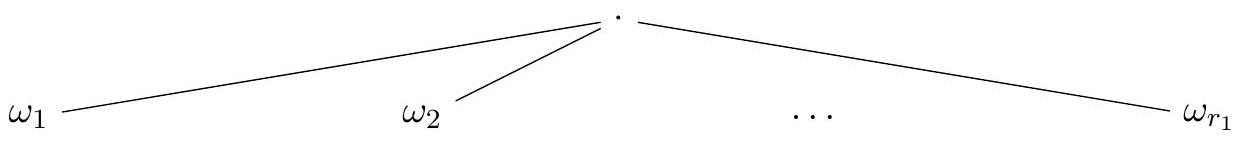
\includegraphics[alt={},max width=\textwidth]{63c8d736-eef8-427f-89a9-bfd33161edc8-09_144_1241_2134_440}
\captionsetup{labelformat=empty}
\caption{Figure 1: The first level partition}
\end{center}
\end{figure}

Then the branches from each child of $\Omega_{1}$ on the first level will be the orbit representatives on the second level, such that for fixed $\Omega_{1}=\omega_{i}$ we get orbit representatives $\left\{v_{j}^{i}: \omega_{i} \mapsto \omega_{i}\right\}$ for $1 \leq j \leq r_{2}^{i}$.

Where for the partition on the second level we use the subset of $\mathcal{L}$, that maps $\Omega_{1}$ to itself, defined in (9) and denoted as $\mathcal{L}_{\Omega_{1}}, \forall \Omega_{1}=\omega_{i} \in\left\{\omega_{1}, \ldots, \omega_{r_{1}}\right\}: \mathbb{F}_{2^{n}}=\operatorname{Orb}\left(v_{1}^{i}, \mathcal{L}_{\omega_{i}}\right) \cup \cdots \cup \operatorname{Orb}\left(v_{r_{2}^{i}}^{i}, \mathcal{L}_{\omega_{i}}\right)$.

\begin{figure}[h]
\begin{center}
  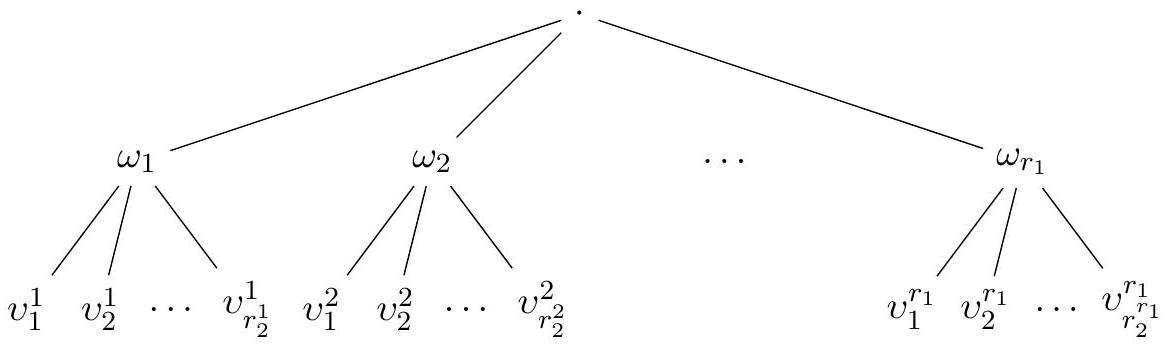
\includegraphics[alt={},max width=\textwidth]{63c8d736-eef8-427f-89a9-bfd33161edc8-10_344_1166_408_476}
\captionsetup{labelformat=empty}
\caption{Figure 2: The second level partition}
\end{center}
\end{figure}

We can see that such a partition can be performed for as many levels $k$ as we want, but the deeper down we partition, the more variables we need to fix in the linear mapping. As a result, fewer and fewer linear permutations will take part in the partitioning, and the number of orbit representatives will get closer to $2^{n}-1$. That is why we need to stop the process of partitioning to the level where it starts to be useless. By recursively traversing the orbit tree and counting the number of leaves, we can calculate an upper bound on the number of matrices to be checked.

\begin{verbatim}
Algorithm 4 Estimate Tree Size
    function EstimateTs( $\mathcal{L}$, level, number_of_variables, max_classes)
        - $\mathcal{L}$ : Set of linear permutations; level: current level, number_of_variables: total number of
    variables; max_classes: max number of classes; $n$ : is a global variable for dimension.
    /* Check if we are in a leaf */
        if level $\geq$ number_of_variables then
            return 1
        end if
        total_size ← 0
    /* Partition according to $\mathcal{L}^{*} /$
        classes $\leftarrow \operatorname{FindLinear}(\mathcal{L})$
        reps $\leftarrow$ EQUIVSet(classes)
    /* Check termination condition */
        if \#classes > max_classes then
            return $\left(2^{n}\right)^{\text {number_of_variables-level }-1} \times$ \#classes
        end if
    /* Handle sub-tree recursively */
        for $v$ in reps do
            $\mathcal{L}_{v} \leftarrow\{l \in \mathcal{L} \mid l(v)=v\}$
            total_size ← total_size + EstimateTs $\left(\mathcal{L}_{v}\right.$, level +1 , number_of_variables, max_classes $)$
        end for
        return total_size
    end function
\end{verbatim}

We start with the partition on the first level, where we get orbit representatives $\left\{\omega_{1}, \ldots, \omega_{r_{1}}\right\}$. We then traverse them and define $\left\{\left(\omega_{i}, v_{j}^{i}\right)\right\}_{i, j}$, where $i=\left\{1, \ldots, r_{1}\right\}$ and $j=\left\{r_{2}^{i}\right\}_{i}$ is a different number of orbit representative for each $i$, both $r_{1}, r_{2}$ do not exceed ( $2^{n}-1$ ). Until some level\\
$k<r$ we find it inefficient and stop partitioning. We have chosen $2^{n-1}+2^{n-2}$ to be the number close to the $\left(2^{n}-1\right)$ when we stop partitioning. Therefore we repeat the process of traversing and partitioning recursively until the level $k-1$ inclusively, then backtrack and count the number of leaves, see an Algorithm 4.

\subsection*{3.4 Submatrix test}
In the computational search, we guess variables level by level. Applying orbit partitioning on each level makes the search space smaller, yet we need more restrictions to make the search faster.

When we search for new APN functions using derivative matrices, we can use submatrices to reduce the number of matrices that we have to check for being QAM as was done in [15].

Let $M_{F} \in \mathbb{F}_{2^{n}}^{n \times n}$ be a derivative matrix of some function $F$ of the form (1). The matrix $M_{F}$ is QAM if and only if for every $1 \leq p, q \leq n$ every submatrix $S \in \mathbb{F}_{2^{n}}^{p \times q}$ of $M_{F}$ is proper.

Definition 3.1. [15] $S$ is proper if every nonzero linear combinations of the $p$ rows has rank at least $q-1$.

Starting from the second level, we can already completely determine some submatrices, and check if they are proper. It helps to cut off branches of the search tree that will never lead to a QAM regardless of the instantiation of the remaining variables [7]. We check the condition of the submatrices for being proper on each level (except the last one) in our depth-first search. Moreover, we pre-generate the set of indices for submatrices for each level, avoiding repetitions, indices that produce equivalent matrices, etc. We also use Theorem 2 to reduce the number of indices for each level, making the submatrix test work faster.

To the best of our knowledge, only "left-side" equivalence (described in Section 3.1) was applied for the QAM method, as it is difficult to say anything about the effect of composing on the right. Despite this, we make the following observation:

Theorem 2. Let us fix a normal basis $\mathcal{B}=\left\{b, b^{2}, \ldots, b^{2^{n-1}}\right\}$ of $\mathbb{F}_{2^{n}}$ over $\mathbb{F}_{2}$. If $M_{F}(\mathcal{B})=M_{F}= \left(M_{i, j}\right)_{1 \leq i, j \leq n}$ is the derivative matrix (5) of the quadratic function $F$ then the matrix $M_{F^{\prime}}= \left(M_{\sigma(i), \sigma(j)}\right)_{1 \leq i, j \leq n}$ will be the derivative matrix of the equivalent function $F^{\prime}=F \circ L$, where $L= \alpha x^{2^{s}}$, for any $\alpha \in \mathbb{F}_{2^{m}}$. Here $\sigma_{s}(i)$ represents a cyclic shift of rows and columns on $i$, i.e. $\sigma_{s}(i)= i+s, s \in\{0, \ldots, n-1\}$, when $\sigma_{s}(i)>n$, we take $\sigma_{s}(i) \bmod n$.

Proof. For a fixed basis with a normal element $b \in \mathbb{F}_{2^{n}}$, the structure of the derivative matrix $M_{F}$ of a function $F(x)=\sum_{i=0}^{n-1} c_{i} x^{i}$, where $c_{i} \in \mathbb{F}_{2^{m}}$, is given by (5) as $M_{F}=\left(\Delta F\left(b^{2^{i}}, b^{2^{j}}\right)\right)_{1 \leq i, j \leq n}$.

For a function $F^{\prime}=F\left(\alpha x^{2^{s}}\right)$, where $\alpha \in \mathbb{F}_{2^{m}}$, its symmetric derivative (2) in the direction $a \in \mathbb{F}_{2^{n}}$ :

$$
\Delta F^{\prime}(a, x)=F\left(\alpha(a+x)^{2^{s}}\right)+F\left(\alpha x^{2^{s}}\right)+F\left(\alpha a^{2^{s}}\right)+F(0)
$$

which is $\Delta F^{\prime}(a, x)=\Delta F\left(\alpha a^{2^{s}}, \alpha x^{2^{s}}\right)$. It shows that

$$
M_{F^{\prime}}=\left(\Delta F\left(\alpha b^{2^{(i+s)}}, \alpha b^{2^{(j+s)}}\right)\right)_{1 \leq i, j \leq n}
$$

Since $\alpha$ is a constant in $\mathbb{F}_{2^{n}}$, it can be factored out, and the structure of the matrix depends only on the powers of $b$. The effect of the transformation is a cyclic shift of the indices $i$ and $j$ by $s$, which corresponds to the shift $\sigma_{s}(i)=i+s$.

This gives us invariance of QAM property under the cyclic shifts for rows and columns. We use this property to reduce the set of submatrices for the test on each level of the search. For example, we can omit the check of submatrices produced from the conjugates of already checked submatrix. It makes the search much faster, see Section 5.3 for example. Moreover, this is true for any quadratic function without the restriction on its coefficients. Examples of application of the theorem outside the submatrix test can be found in Subsection 4.5.1.

\subsection*{3.5 Reducing number of linear combinations for QAM check}
Set a normal basis $\mathcal{B}=\left\{b, b^{2}, \ldots, b^{2^{n-1}}\right\}$ of $\mathbb{F}_{2^{n}}$ over $\mathbb{F}_{2}$. Let $M_{F}(\mathcal{B}) \in \mathbb{F}_{2^{n}}^{n \times n}$ be a derivative matrix (5) of the quadratic function $F(x)=\sum_{0 \leq i<j \leq n-1} a_{i, j} x^{2^{i}+2^{j}}$ over $\mathbb{F}_{2^{n}}$ with coefficients $a_{i, j}$ in the subfield $\mathbb{F}_{2^{m}}$. Represent $M_{F}$ using the row vector decomposition $M_{F}(\mathcal{B})=\left(r_{1}, r_{2}, \ldots, r_{n}\right)^{T}$, where each row vector $r_{i}=\left(r_{i 1}, r_{i 2}, \ldots, r_{i n}\right) \in \mathbb{F}_{2^{n}}^{n}$, we can generalize the Theorem 2 from [12]:

Theorem 3. Any non-zero linear combination $\left\{\alpha_{i} r_{i}\right\}_{i=1}^{n}$ of rows will have the same rank as the same linear combination of cyclically shifted rows $\left\{\alpha_{i} r_{i+m}\right\}_{i=1}^{n}$, that is

$$
\operatorname{Rank}\left(\sum_{i=1}^{n} \alpha_{i} r_{i+m}\right)=\operatorname{Rank}\left(\sum_{i=1}^{n} \alpha_{i} r_{i}\right),
$$

for any $\alpha=\left(\alpha_{1}, \ldots, \alpha_{n}\right) \in \mathbb{F}_{2}^{n}$, when $i+m>n$, we take $i+m \bmod n$.\\
Proof. Using the diagonalization property (6) of the matrix $M_{F}$, we have that each element in the span of linear combinations of the rows of $M_{F}$ is mapped to a cyclically shifted element when raised to the power $2^{m}$. Specifically, for any linear combination of rows, we have:

$$
\operatorname{Span}\left(\sum_{i=1}^{n} \alpha_{i} r_{i+m}\right)=\operatorname{Span}\left(\sum_{i=1}^{n} \alpha_{i} r_{i}^{2^{m}}\right), \text { for } \alpha_{i} \in \mathbb{F}_{2}
$$

Which means that $\operatorname{Rank}\left(\sum_{i=1}^{n} \alpha_{i} r_{i+m}\right)=\operatorname{Rank}\left(\sum_{i=1}^{n} \alpha_{i} r_{i}^{2^{m}}\right)=\operatorname{Rank}\left(\sum_{i=1}^{n} \alpha_{i} r_{i}\right)$.

We apply this theorem to the algorithm that checks whether a constructed matrix is QAM, where instead of checking all possible linear combinations of rows, we exclude those that have the same rank. This accelerates the QAM check significantly, for example, in the case $(n, m)=(10,2)$ checking if all linear combinations of the matrix have the rank $n-1$ takes on average 0.08 seconds, while only 0.04 seconds applying Theorem 3 (on the server with 64 GB of RAM, and 32 VCPUs). This was tested on QAM matrices, as non-QAM tests terminate quickly.

\section*{4 Applying improved QAM method to the particular cases}
In this section, we apply the approaches described above to the particular cases of the quadratic functions $F(x)=\sum_{0 \leq i<j \leq n-1} a_{i, j} x^{2^{i}+2^{j}}$ over $\mathbb{F}_{2^{n}}$ with coefficients $a_{i, j}$ in the subfield $\mathbb{F}_{2^{m}}$.

\section*{$4.1 \quad(n, m)=(8,2)$}
Let us set a normal basis $\left\{b, b^{2}, \ldots, b^{2^{7}}\right\}$ of $\mathbb{F}_{2^{8}}$ over $\mathbb{F}_{2}$, where $b$ is a normal element. Considering homogeneous quadratic functions $F: \mathbb{F}_{2^{8}} \rightarrow \mathbb{F}_{2^{8}}$ with coefficients in the subfield $\mathbb{F}_{2^{2}}$, we can construct its derivative matrix $M \in \mathbb{F}_{2^{8}}^{8 \times 8}$ using (5). The structure of $M$ follows a diagonalization property (6) for $m=2$ :

$$
M_{i+2, j+2}=\left(M_{i, j}\right)^{2^{2}}
$$

where $1 \leq i, j \leq n$, and when we get an index that exceeds the size of the matrix we modulate it with 8 . For example, taking the entry $i=1, j=2$, where the first variable $\Omega_{1}$ is located, we get:

$$
M_{3,4}=\left(M_{1,2}\right)^{4}, M_{5,6}=\left(M_{3,4}\right)^{4}, M_{7,8}=\left(M_{5,6}\right)^{4}, M_{1,2}=\left(M_{7,8}\right)^{4}
$$

Continuing doing the same for the variables $\Omega_{2}, \ldots \Omega_{8}$ step-by-step, we can see that it is enough to have 8 unknowns to fill the whole matrix. Note, that we fill variables from the first row further down, depending on the availability of the entry. For example, entry $M_{1,7}$ is already taken by the variable $\Omega_{2}$, s.t. $M_{1,7}=\left(\Omega_{2}\right)^{2}$, therefore we placed $\Omega_{6}$ on the "non-taken" entry $M_{1,8}$. As long as we have only 8 variables, we can use letters in alphabetical order $A, B, C, D, E, F, G, H$ for convenience:

\[
M=\left[\begin{array}{cccccccc}
0 & A & B & C & D & E & B^{2^{6}} & F  \tag{11}\\
A & 0 & F^{2^{2}} & G & E^{2^{4}} & H & C^{2^{6}} & G^{2^{6}} \\
B & F^{2^{2}} & 0 & A^{2^{2}} & B^{2^{2}} & C^{2^{2}} & D^{2^{2}} & E^{2^{2}} \\
C & G & A^{2^{2}} & 0 & F^{2^{4}} & G^{2^{2}} & E^{2^{6}} & H^{2^{2}} \\
D & E^{2^{4}} & B^{2^{2}} & F^{2^{4}} & 0 & A^{2^{4}} & B^{2^{4}} & C^{2^{4}} \\
E & H & C^{2^{2}} & G^{2^{2}} & A^{2^{4}} & 0 & F^{2^{6}} & G^{2^{4}} \\
B^{2^{6}} & C^{2^{6}} & D^{2^{2}} & E^{2^{6}} & B^{2^{4}} & F^{2^{6}} & 0 & A^{2^{6}} \\
F & G^{2^{6}} & E^{2^{2}} & H^{2^{2}} & C^{2^{4}} & G^{2^{4}} & A^{2^{6}} & 0
\end{array}\right] .
\]

The variables $A, B, C, E, F, G$ can take any value of $\mathbb{F}_{2^{8}} \backslash\{0\}$, and $D, H \in \mathbb{F}_{2^{4}} \backslash\{0\}$ as we have $D=D^{2^{4}}$ and $H=H^{2^{4}}$.

Brute-forcing through $A, B, C, D, E, F, G, H$ for checking if the derivative matrix $M$ is QAM, would require a test of $255^{6} \times 15^{2} \approx 6.19 \times 10^{16}$ different matrices. It takes approximately 0.010 seconds at most on our server to check an $8 \times 8$ matrix for being QAM, which means that performing a test for all possible matrices without placing any restrictions on the search would take approximately $6.19 \times 10^{15}$ seconds, or 196283612 years.

To use the orbit restriction described in the previous section, firstly, we found all linear permutations over $\mathbb{F}_{2^{8}}$ with the coefficients in $\mathbb{F}_{2^{2}}$. The set of all these permutations $\mathcal{L}$ has cardinality 24576. Let $a$ be the primitive element in $\mathbb{F}_{2^{8}}$ corresponding to the primitive polynomial $x^{8}+x^{4}+x^{3}+x^{2}+1$. Applying $\mathcal{L}$ we get an orbit partition of the field on the first level, using the Algorithm 1:

$$
\mathbb{F}_{2^{8}}=\operatorname{Orb}(1, \mathcal{L}) \cup \operatorname{Orb}(a, \mathcal{L}) \cup \operatorname{Orb}\left(a^{7}, \mathcal{L}\right) \cup \operatorname{Orb}\left(a^{17}, \mathcal{L}\right)
$$

Thus, instead of brute-forcing $A$ through all $2^{8}-1$ elements, we will only consider 4 elements of the field - one representative from each orbit (Algorithm 2), i.e.

$$
\mathcal{A}=\left\{1, a, a^{7}, a^{17}\right\} .
$$

We choose the orbit representative so that it has the lowest exponent of the primitive element in the orbit. Also, we denote the set of orbit representatives by a calligraphic letter depending on the variable we are brute-forcing through, which is $A$ in our case. Continuing further down the orbit tree, we get different partitions for each variable $A \in\left\{1, a, a^{7}, a^{17}\right\}$. For example, for $A=1$ we get the next partition using linear permutations from $\mathcal{L}$ that map 1 to itself:

$$
\begin{aligned}
\mathbb{F}_{2^{8}}=\operatorname{Orb}_{1}(1, \mathcal{L}) \cup \operatorname{Orb}_{1}(a, \mathcal{L}) & \cup \operatorname{Orb}_{1}\left(a^{5}, \mathcal{L}\right) \cup \operatorname{Orb}_{1}\left(a^{7}, \mathcal{L}\right) \cup \operatorname{Orb}_{1}\left(a^{13}, \mathcal{L}\right) \cup \\
& \cup \operatorname{Orb}_{1}\left(a^{17}, \mathcal{L}\right) \cup \operatorname{Orb}_{1}\left(a^{51}, \mathcal{L}\right) \cup \operatorname{Orb}_{1}\left(a^{85}, \mathcal{L}\right)
\end{aligned}
$$

Therefore, instead of brute-forcing the second variable $B$ through all possible elements of the field, we can only check orbit representatives

$$
\mathcal{B}_{1}=\left\{1, a, a^{5}, a^{7}, a^{13}, a^{17}, a^{51}, a^{85}\right\}
$$

We use calligraphic $B$ in this case which corresponds to the variable name, and the same index as the orbit representative. The index corresponds to the element chosen on the previous level that maps to itself in the current partition, for our example $l(1)=1, l \in \mathcal{L}$.

Continuing to the third variable $C$ for chosen $B=a$ and $A=1$, the partition is

$$
\mathbb{F}_{2^{8}}=\operatorname{Orb}_{1, a}(1, \mathcal{L}) \cup \operatorname{Orb}_{1, a}(a, \mathcal{L}) \cup \cdots \cup \operatorname{Or} b_{1, a}\left(a^{224}, \mathcal{L}\right),
$$

it has 30 orbits, correspondingly 30 orbit representatives

$$
\mathcal{C}_{1, a}=\left\{1, a, a^{2}, a^{3}, \ldots, a^{224}\right\} .
$$

This is again significantly fewer than 255 elements for an exhaustive search.\\
We are interested in orbit representatives, moreover in the number of them, to estimate the time the search will take.

As we can see from the example, $\# \mathcal{A}=4$ which is 4 orbit representatives on the first level, then $\# \mathcal{B}_{1}=8$ on the second level for fixed $A=1$. When we computed orbits for the third level there are $\# \mathcal{C}_{1, a}=30$ while if we chose $B=a^{85}$ branch we will get $\# \mathcal{C}_{1, a^{85}}=12$, see Figure 3.

\begin{figure}[h]
\begin{center}
  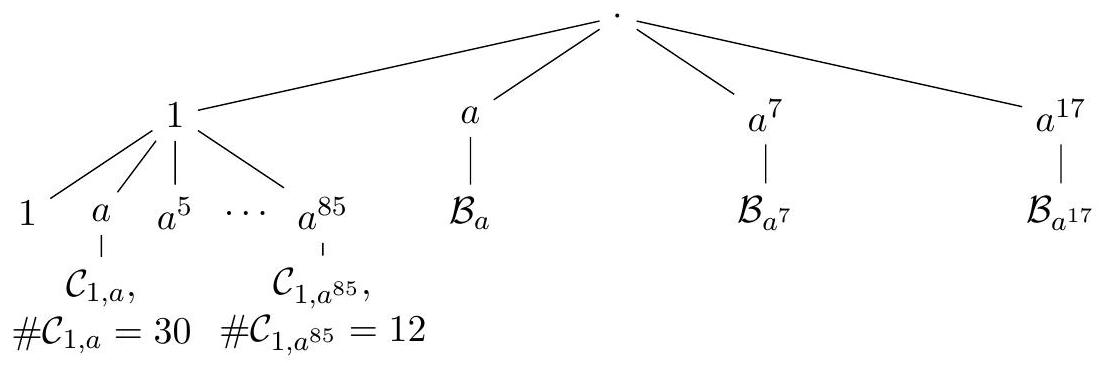
\includegraphics[alt={},max width=\textwidth]{63c8d736-eef8-427f-89a9-bfd33161edc8-14_366_1103_1607_509}
\captionsetup{labelformat=empty}
\caption{Figure 3: The number of orbits for every branch on the first three levels for $(n, m)=(8,2)$}
\end{center}
\end{figure}

The orbit tree expands quickly, and we have different cardinalities for $\mathcal{C}_{1, B}$ depending on the choice of $B \in \mathcal{B}_{1}$. We can take the average number of orbits created on the third level, as in Table 1.

From the table, we see that the number of orbits increases significantly. Some branches of the orbit tree take longer to search through, therefore an average time interval taken will not necessarily give an accurate measurement. Therefore, we will use Algorithm 4 for an upper bound on the total number of matrices for our search. We could exhaust the whole dimension and describe computational results in the next section.

\begin{table}[h]
\begin{center}
\begin{tabular}{c|c|c}
$A$ & Number of orbits of $B$ & Average number of orbits of $C$ \\
\hline
1 & 8 & 22.1 \\
$a$ & 30 & 56.7 \\
$a^{7}$ & 22 & 43.5 \\
$a^{17}$ & 14 & 41.5 \\
\end{tabular}
\captionsetup{labelformat=empty}
\caption{Table 1: Representative elements of the orbits of $A$, the number of orbits of $B$ and the average number of orbits of $C$, taken over all orbits of $B$}
\end{center}
\end{table}

\section*{$4.2(n, m)=(8,4)$}
Performing the same steps as in the previous subsection, yet for quadratic functions over $\mathbb{F}_{2}$ with coefficients in $\mathbb{F}_{2^{4}}$, we get the structure of the derivative matrix $M$ with $M_{i+4, j+4}=\left(M_{i, j}\right)^{2^{4}}$. Therefore, the general representation of the derivative matrix for any quadratic function in this case is given by (20), see Appendix A . With $A, B, C, E, F, G, H, I, K, L, M, O \in \mathbb{F}_{2^{8}}$, and $D, J, N, P \in \mathbb{F}_{2^{4}}-16$ variables for depth-first in total.

The set $\mathcal{L}$ of all lineal permutations over $\mathbb{F}_{2^{8}}$ with coefficients in the subfield $\mathbb{F}_{2^{4}}$ is infeasible for generation with current computational needs, therefore we use Theorem 1 for partition. Any nonzero elements of the field $\alpha \in \mathbb{F}_{2^{n}}$ can be categorized into cases:

\begin{itemize}
  \item $\operatorname{Cat}_{1}=\left\{\alpha: \alpha \in \mathbb{F}_{2^{8}} \backslash\{0\} \mid \alpha+\alpha^{2^{4}}=0\right\}$,
  \item $\operatorname{Cat}_{\text {Ind }}=\left\{\alpha: \alpha \in \mathbb{F}_{2^{8}} \backslash\{0\} \mid \alpha \notin C a t_{1}\right\}$.
\end{itemize}

By applying Theorem 1 to the elements in $C a t_{\text {Ind }}$, we get if there exists a linear function that maps $\alpha \mapsto \beta$, then $\alpha$ and $\beta$ belong to the same orbit, which forms an equivalent class. Thus, we can denote this relationship as $\alpha \sim \beta$ for convenience. Leveraging an algorithm built using Theorem 1 and Lemma 1 we obtain:

$$
\mathcal{A}=C a t_{1} \cup\{a\} ;
$$

Moreover, we can generalize Theorem 1 for the case of one or more fixed variables. Let us set $A$ on the first level, then to partition the second level, we suggest the following proposition:\\
Proposition 1. 1. For $A \in$ Cat $_{\text {Ind }}$, if there exist a linear function $l(x)=\sum_{i=0}^{7} c_{i} x^{2^{i}}, c_{i} \in \mathbb{F}_{2^{4}}$ s.t. $l(\alpha)=\beta, l(A)=A$; then there exist a linear permutation $l^{\prime}$, s.t. $l^{\prime}(A)=A, l^{\prime}(\alpha)=\beta$.\\
2. For $A \in C a t_{1}$, if there exist $l(x)=\sum_{i=0}^{7} c_{i} x^{2^{i}}, c_{i} \in \mathbb{F}_{2^{4}}$ s.t. $l(\alpha)=\beta, l(\beta)=\alpha, l(A)=A$; then there exist a linear permutation $l^{\prime}$, s.t. $l^{\prime}(A)=A$, $l^{\prime}(\alpha)=\beta$.

Proof. 1. $A \in C a t_{\text {Ind }}$. With the linear function $l$, we get the mappings:

$$
A \mapsto A ; A^{2^{4}} \mapsto A^{2^{4}} ; \alpha \mapsto \beta ; \alpha^{2^{4}} \mapsto \beta^{2^{4}} .
$$

We consider $\alpha$ and $\beta$ to belong to the same category, as we automatically assign elements to different orbits if they belong to the different categories (Lemma 1).

\begin{itemize}
  \item In the case $\alpha, \beta \in \operatorname{Cat}_{\text {Ind }}$, we obtain a linearly independent set $\left\{A, A^{2^{4}}, \alpha, \alpha^{2^{4}}\right\}$ which can be extended to the basis, proving the existence of the linear permutation.
  \item In the case $\alpha, \beta \in C a t_{1}$, we get $A \mapsto A ; A^{2^{4}} \mapsto A^{2^{4}} ; \alpha \mapsto \beta$. Let $\left\{A, A^{2^{4}}, \alpha\right\}$ be linearly dependent, then $A+A^{2^{4}}=\alpha$, applying a linear mapping on both sides, we get $l(A)+ l\left(A^{2^{4}}\right)=l(\alpha)$, so $A+A^{2^{4}}=\beta$, leading to $\alpha=\beta$, where an identity permutation exist; otherwise $\left\{A, A^{2^{4}}, \alpha\right\}$ is linearly independent. Therefore this mapping can similarly be extended to a basis, yielding the desired linear permutation.
\end{itemize}

\begin{enumerate}
  \setcounter{enumi}{1}
  \item $A \in C a t_{1}$. With the linear function $l$, we get the mappings:
\end{enumerate}

$$
A \mapsto A ; \alpha \mapsto \beta ; \alpha^{2^{4}} \mapsto \beta^{2^{4}} ; \beta \mapsto \alpha ; \beta^{2^{4}} \mapsto \alpha^{2^{4}} ;
$$

\begin{itemize}
  \item Let $\alpha, \beta \in C a t_{\text {Ind }}$, consider $\nu_{0} A+\nu_{1} \alpha+\nu_{2} \alpha^{2^{4}}+\nu_{3} \beta+\nu_{4} \beta^{2^{4}}=0, \nu_{i} \in \mathbb{F}_{2}$. Here $\nu_{0} \neq 0$, as $\alpha, \beta \in C a t_{\text {Ind }}$, so $A=\nu_{1} \alpha+\nu_{2} \alpha^{2^{4}}+\nu_{3} \beta+\nu_{4} \beta^{2^{4}}$.\\
Applying $l$ on both sides, we get $A=\nu_{1} \beta+\nu_{2} \beta^{2^{4}}+\nu_{3} \alpha+\nu_{4} \alpha^{2^{4}}$, leading to $\left(\nu_{1}+\nu_{3}\right)(\alpha+\beta)+\left(\nu_{2}+\nu_{4}\right)\left(\alpha^{2^{4}}+\beta^{2^{4}}\right)=0$, giving $\alpha=\beta$, or $(\alpha+\beta)^{15}=1$ which is impossible as $\alpha, \beta \in \operatorname{Cat}_{\text {Ind }}$. Therefore $\left\{A, \alpha, \alpha^{2^{4}}, \beta, \beta^{2^{4}}\right\}$ is linearly independent.
  \item In the case $\alpha, \beta \in C a t_{1}$, we get $A \mapsto A ; \alpha \mapsto \beta ; \beta \mapsto \alpha$. Consider $\nu_{0} A+\nu_{1} \alpha+\nu_{2} \beta=0$, without the loss of generality, we take $\nu_{0}=1$, as all three are distinct. Apply $l$ on both sides: $A=\nu_{1} \beta+\nu_{2} \alpha$, so $\left(\nu_{1}+\nu_{2}\right)(\alpha+\beta)=0$ leads to contradiction.
\end{itemize}

Continuing forward, we can get a general method for partitioning for variables $\Omega_{i}$.\\
Proposition 2. For $\Omega_{1}, \Omega_{2}, \ldots, \Omega_{k} \in$ Cat $_{\text {Ind }}$. After we fixed $k$ variables, in order to partition $k+1$-level:

\begin{enumerate}
  \item Choose $\Omega_{k+1} \in$ Cat $_{\text {Ind }}$ s.t. $\left\{\Omega_{1}, \ldots, \Omega_{k+1}\right\}$ - linearly independent set of vectors;
  \item Then $\forall \alpha, \beta \in \mathbb{F}_{2^{n}}: \alpha \sim \beta$, if there exist $l(x)=\sum_{i=0}^{7} c_{i} x^{2^{i}}, c_{i} \in \mathbb{F}_{2^{4}}$ s.t. $l(\alpha)=\beta, l(\beta)= \alpha, \forall i \in\{1, \ldots, k+1\}: l\left(\Omega_{i}\right)=\Omega_{i}$.
\end{enumerate}

Using Proposition 1,2 together with Theorem 1, and Lemma 1 - we performed the next partition for 8 levels of the orbit tree, see Figure 4.

\begin{figure}[h]
\begin{center}
  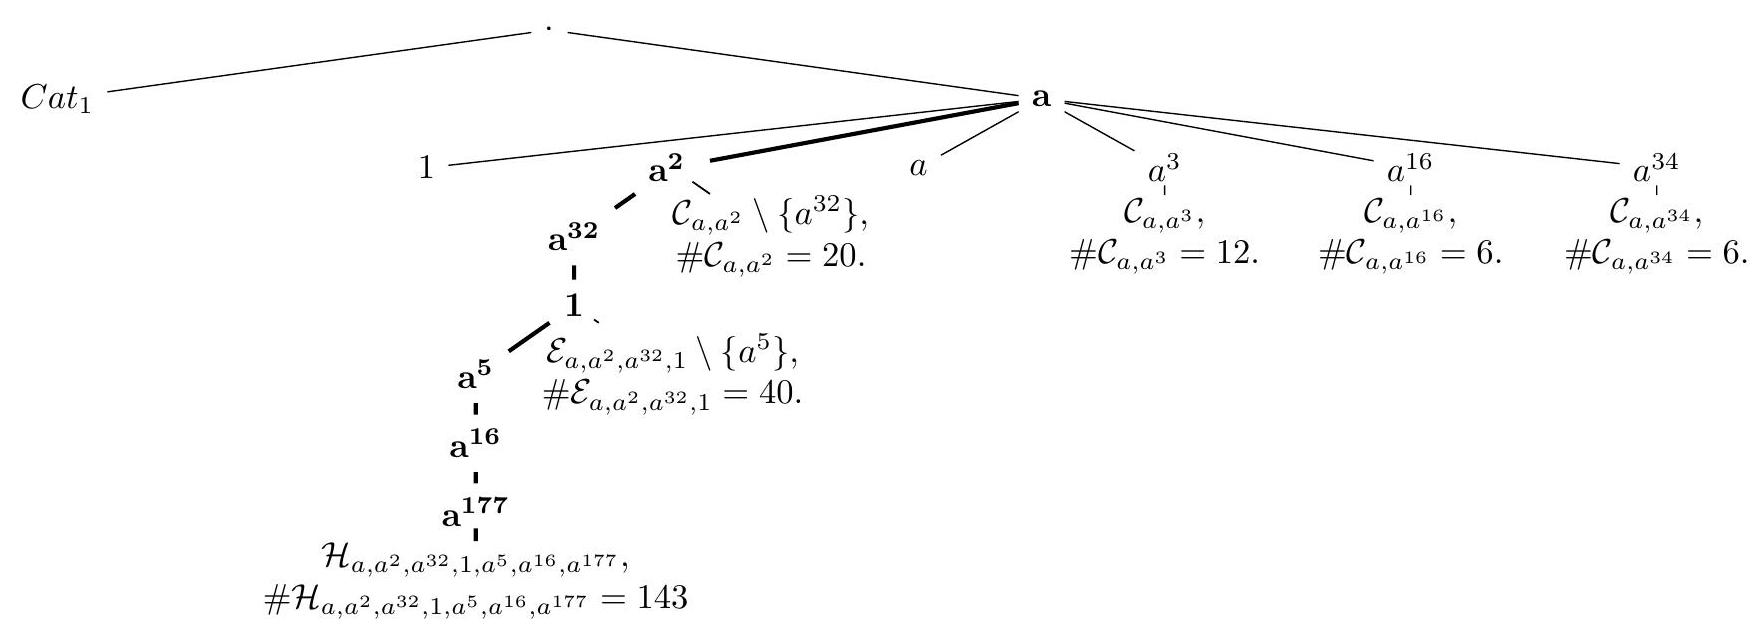
\includegraphics[alt={},max width=\textwidth]{63c8d736-eef8-427f-89a9-bfd33161edc8-16_635_1763_1501_242}
\captionsetup{labelformat=empty}
\caption{Figure 4: The partition for $(n, m)=(8,4)$}
\end{center}
\end{figure}

Let us fix the first 8 levels such that $A=a, B=a^{2}, C=a^{32}, D=1, E=a^{5}, F=a^{16} ; G= a^{177}$. For this choice of branch, there are 143 candidates for the next level variable $H$. We perform a partial search for this case and describe it in the next section.

\section*{$4.3 \quad(n, m)=(9,3)$}
Following the same approach as in the previous subsection for quadratic functions over $\mathbb{F}_{2^{9}}$ with coefficients in $\mathbb{F}_{2^{3}}$, we get the derivative matrix that has 12 variables: $A, B, C, D, E, F, G, H, I, J, K, L \in \mathbb{F}_{2^{9}}$. For the structure of the derivative matrix $M$ see (21) in Appendix A.

In this dimension, the set $\mathcal{L}$ of all linear permutations with coefficients in the subfield is also unfeasible for pre-generation. Therefore, we use Theorem 1 for partition. Elements of the field can be categorized into disjoint sets:

\begin{itemize}
  \item $C a t_{1}=\left\{\alpha \in \mathbb{F}_{2^{9}} \backslash\{0\} \mid \alpha+\alpha^{2^{3}}=0\right\} ;$
  \item Cat $_{2}=\left\{\alpha \in \mathbb{F}_{2^{9}} \backslash\{0\} \mid \alpha+\alpha^{2^{3}}+\alpha^{2^{6}}=0\right\}$;
  \item $\operatorname{Cat}_{\text {Ind }}=\left\{\alpha \in \mathbb{F}_{2^{9}} \backslash\{0\} \mid \alpha \notin \operatorname{Cat}_{1}, \alpha \notin \operatorname{Cat}_{2}\right\}$.
\end{itemize}

To partition the first level we use Theorem 1 and Lemma 1. Then, we fix $A$ on the first level and partition the second level using the following proposition:\\
Proposition 3. For $A \in$ Cat $_{\text {Ind }}$, if there exists a linear function $l(x)=\sum_{i=0}^{8} c_{i} x^{2^{i}}, c_{i}^{\prime} \in \mathbb{F}_{2^{3}}$, s.t. $l(\alpha)=\beta, l(A)=A$; then there exist a linear permutation $l^{\prime}$, s.t. $l^{\prime}(\alpha)=\beta, l^{\prime}(A)=A$.

Proof. $A \in C a t_{\text {Ind }}$. For $\alpha, \beta \in C a t_{\text {Ind }}$, we get linearly independent set of vectors


\begin{equation*}
\left\{A, A^{2^{3}}, A^{2^{6}}, \alpha, \alpha^{2^{3}}, \alpha^{2^{6}}\right\} \tag{12}
\end{equation*}


For the rest of the cases, we consider $\nu_{0} A+\nu_{1} A^{2^{3}}+\nu_{2} A^{2^{6}}=\nu_{3} \alpha+\nu_{4} \alpha^{2^{3}}+\nu_{5} \alpha^{2^{6}}, \nu_{i} \in \mathbb{F}_{2}$. Applying $l$ on both sides: $\nu_{0} A+\nu_{1} A^{2^{3}}+\nu_{2} A^{2^{6}}=\nu_{3} \beta+\nu_{4} \beta^{2^{3}}+\nu_{5} \beta^{2^{6}}, \nu_{i} \in \mathbb{F}_{2}$, leading to $\nu_{3}(\alpha+\beta)+\nu_{4}\left(\alpha^{2^{3}}+\right. \left.\beta^{2^{3}}\right)+\nu_{5}\left(\alpha^{2^{6}}+\beta^{2^{6}}\right)=0$\\
With $\alpha, \beta \in C a t_{1}$, we get the case of $\alpha=\beta$, so (12) is linearly independent.\\
For $\alpha, \beta \in C a t_{2}$, we get $\left(\nu_{3}+\nu_{5}\right)(\alpha+\beta)+\left(\nu_{4}+\nu_{5}\right)\left(\alpha^{2^{3}}+\beta^{2^{3}}\right)=0$, leading to easier $\alpha=\beta$, or $(\alpha+\beta)^{2^{3}-1}=1$, which cannot happen when $\alpha, \beta \in C a t_{2}$, so (12) is linearly independent.

\section*{$4.4(n, m)=(10,1)$}
For the derivative matrix $M$ that correspond to any quadratic function over $\mathbb{F}_{2^{10}}$ with coefficients in the prime field, we have $M_{i+1, j+1}=\left(M_{i, j}\right)^{2}$. The general representation of the matrix will be (22), see Appendix A. We get $A, B, C, D, E-5$ variables, where $A, B, C, D, E \in \mathbb{F}_{2^{10}}$ and $E \in \mathbb{F}_{2^{5}}$, because $\left(M_{6,10}\right)^{2}=E^{2^{5}}=M_{7,1}=E$.

There are just 5 levels in the depth-first search, so the full classification for this case is feasible. Let $a$ be the primitive element of the finite field given by the primitive polynomial $x^{10}+x^{6}+x^{5}+ x^{3}+x^{2}+x+1$. We randomly choose the normal element for the basis of the field $\mathbb{F}_{2^{10}}$ on $\mathbb{F}_{2}$, and fix it to $a^{805}$.

We have $\# \mathcal{L}=480$ linear permutations over $\mathbb{F}_{2^{10}}$ with coefficients in $\mathbb{F}_{2}$, therefore we construct them explicitly. The partition on the first level is $\mathbb{F}_{2^{10}}=\cup_{A \in \mathcal{A}} \operatorname{Orb}(A, \mathcal{L})$, where $a \in \mathcal{A}$ are the orbit representatives as is shown in Figure 5. Thus, instead of brute-forcing $A$ through all $2^{10}-1$ elements, we will only consider 8 elements of the field - one representative from each orbit, i.e.

$$
\mathcal{A}=\left\{1, a, a^{7}, a^{15}, a^{33}, a^{57}, a^{99}, a^{341}\right\}
$$

For every $A \in \mathcal{A}$ we chose a set $\mathcal{L}_{A}$ of permutations from $\mathcal{L}$ that fix $A$, and get orbit representatives $\mathcal{B}_{A}$ by partitioning the second level.

By using the submatrix test, we reduce the number of orbits even more. We also parallelize our code by running each orbit representative in $\mathcal{A}$ separately, detailed description can be found in the next section.

\begin{figure}[h]
\begin{center}
  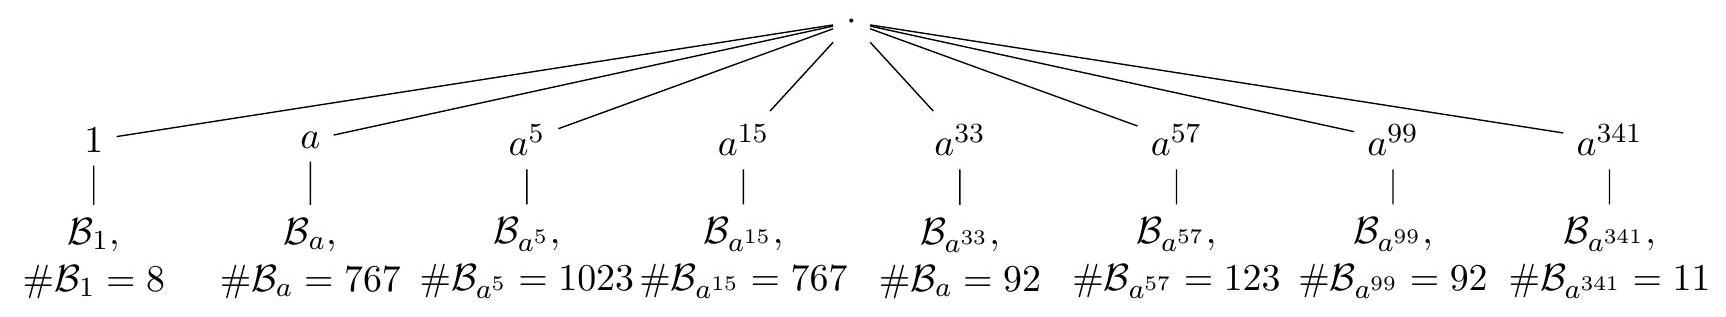
\includegraphics[alt={},max width=\textwidth]{63c8d736-eef8-427f-89a9-bfd33161edc8-18_317_1726_249_240}
\captionsetup{labelformat=empty}
\caption{Figure 5: The number of orbits for every branch on the first two levels for $(n, m)=(10,1)$}
\end{center}
\end{figure}

\section*{$4.5 \quad(n, m)=(10,2)$}
When we take functions over $\mathbb{F}_{2^{10}}$ with coefficients in the $\mathbb{F}_{4}$, the structure of the derivative matrix $M$ has $M_{i+2, j+2}=\left(M_{i, j}\right)^{2^{2}}$ property, and is formulated by (23) in Appendix A. It has 9 variables $A, B, C, D, E, F, G, H, I \in \mathbb{F}_{2^{n}}$ that correspond to each depth-force search level.

For this case, we could generate the set $\mathcal{L}$ using the server with 500 GB of memory, where it is also possible to partition with Theorem 1 for servers with lower RAM. We got $|\mathcal{L}|=367200$ that together with the Algorithm 1 and the Algorithm 2 gave us next partition on the first level:

$$
\mathcal{A}=\left\{1, a, a^{5}\right\} .
$$

Partitioning the second level, we got 5 orbits for $A=1$, only 3 of which passed the submatrix test, we again denote the $\mathcal{B}_{A}=\operatorname{Orb}_{A}=\{l(\alpha): l \in \mathcal{L} \mid l(A) \mapsto A\}$, and with $\mathcal{B}_{A}^{\text {Sub }}$ - the subset of elements from $\mathcal{B}_{A}$ that passed the submatrix test. Similarly, we get partition for $A=a$ and $A=a^{5}$, and further down, see Figure 6.

\begin{figure}[h]
\begin{center}
  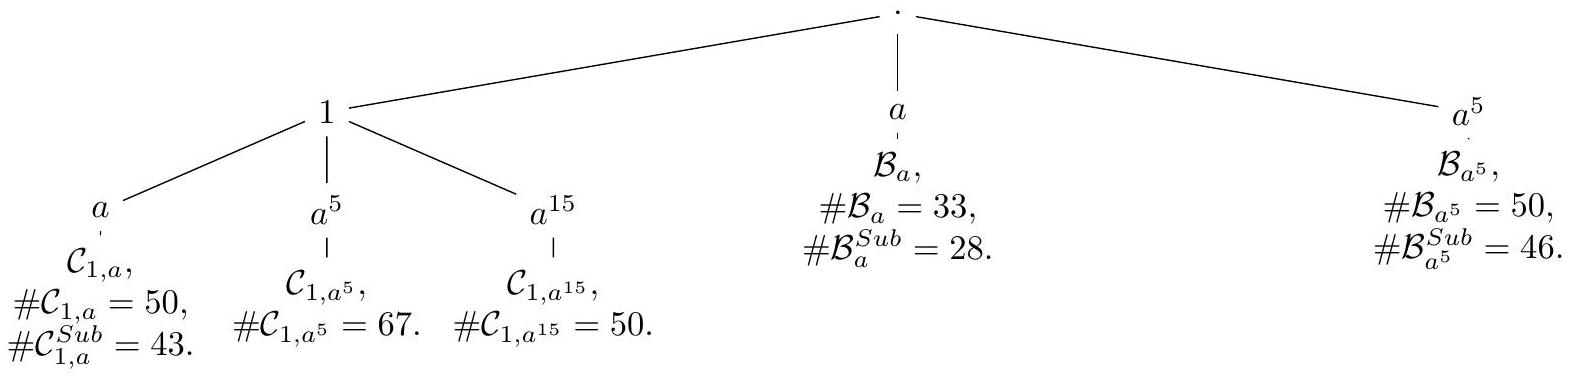
\includegraphics[alt={},max width=\textwidth]{63c8d736-eef8-427f-89a9-bfd33161edc8-18_377_1573_1426_277}
\captionsetup{labelformat=empty}
\caption{Figure 6: The number of orbits for every branch for the first two levels for $(n, m)=(10,2)$}
\end{center}
\end{figure}

The number of orbits increases on each level significantly, which makes partitioning on levels 6 to 9 inefficient. Bruteforcing the last 4 levels takes an infeasible amount of time. We ran the search for more than 3 months without finding any APN functions, therefore we have chosen the partial searches, and explain them in the next section.

\subsection*{4.5.1 Equivalence on the right}
Let $F(x)$ be any purely quadratic function over $\mathbb{F}_{2^{10}}$ with coefficients in $\mathbb{F}_{4}$ with derivative matrix $M_{F(x)}=M$ of the form (23). As $\{A, \ldots, I\}$ is an ordered set of variables that define the structure of $M$, we will denote the derivative matrix with $\operatorname{DerMatr}(A, B, C, D, E, F, G, H, I)$.

Let us take $F^{(s)}(x)=F(x) \circ \alpha x^{2^{s}}$, for any $\alpha \in \mathbb{F}_{4}, s \in\{0, \ldots, 9\}$. Using Theorem 2, the derivative matrix $M_{F^{(s)}(x)}=M^{(s)}$ of the equivalent function can be obtained by performing shifts $\sigma_{s}(i)$ for the derivative matrix $M_{F(x)}=M$ of the original function, i.e.

$$
M^{(s)}=\left(M_{\sigma_{s}(i), \sigma_{s}(j)}\right)_{1 \leq i, j \leq 10}, \text { where } \sigma_{s}(i)=i+s \text {. }
$$

For example, when $s=1$ we get $F^{(1)}=F(x) \circ \alpha x^{2}$, for any $\alpha \in \mathbb{F}_{4}$, and its derivative matrix can be obtained by shift of 1 row and column, see (24) in Appendix A. Specifically, the first row and first column of the original matrix are moved to the last row and the last column while the rest was shifted up: $M_{i, j}^{(1)}=\left(M_{i+1, j+1}\right)_{1 \leq i, j \leq 10}$. We apply $i+1 \bmod n(j+1 \bmod n)$, when $i+1 (j+1)$ exceeds $n$. It is not hard to notice that $M^{(1)}=\operatorname{DerMatr}\left(G^{4}, H, F^{16}, I, E^{64}, C^{256}, A, B^{4}, D^{4}\right)$. All equivalent matrices will look like :

\begin{table}[h]
\begin{center}
\begin{tabular}{|l|l|l|}
\hline
$F(x)$ & M & $\operatorname{DerMatr}(A, B, C, D, E, F, G, H, I)$ \\
\hline
$F(x) \circ \alpha x^{2}$ & $M^{(1)}$ & DerMatr $\left(G^{4}, H, F^{16}, I, E^{64}, C^{256}, A, B^{4}, D^{4}\right)$ \\
\hline
$F(x) \circ \alpha x^{2^{2}}$ & $M^{(2)}$ & DerMatr $\left(A^{4}, B^{4}, C^{4}, D^{4}, E^{4}, F^{4}, G^{4}, H^{4}, I^{4}\right)$ \\
\hline
$F(x) \circ \alpha x^{2^{3}}$ & $M^{(3)}$ & DerMatr $\left(G^{16}, H^{4}, F^{64}, I^{4}, E^{256}, C, A^{4}, B^{16}, D^{16}\right)$ \\
\hline
$F(x) \circ \alpha x^{2^{4}}$ & $M^{(4)}$ & DerMatr ( $A^{16}, B^{16}, C^{16}, D^{16}, E^{16}, F^{16}, G^{16}, H^{16}, I^{16}$ ) \\
\hline
$F(x) \circ \alpha x^{2^{5}}$ & $M^{(5)}$ & DerMatr $\left(G^{64}, H^{16}, F^{256}, I^{16}, E, C^{4}, A^{16}, B^{64}, D^{64}\right)$ \\
\hline
$F(x) \circ \alpha x^{2^{6}}$ & $M^{(6)}$ & DerMatr $\left(A^{64}, B^{64}, C^{64}, D^{64}, E^{64}, F^{64}, G^{64}, H^{64}, I^{64}\right)$ \\
\hline
$F(x) \circ \alpha x^{2^{7}}$ & $M^{(7)}$ & DerMatr ( $G^{256}, H^{64}, F, I^{64}, E^{4}, C^{16}, A^{64}, B^{256}, D^{256}$ ) \\
\hline
$F(x) \circ \alpha x^{2^{8}}$ & $M^{(8)}$ & DerMatr $\left(A^{256}, B^{256}, C^{256}, D^{256}, E^{256}, F^{256}, G^{256}, H^{256}, I^{256}\right)$ \\
\hline
$F(x) \circ \alpha x^{2^{9}}$ & $M^{(9)}$ & DerMatr $\left(G, H^{256}, F^{4}, I^{256}, E^{16}, C^{64}, A^{256}, B, D\right)$ \\
\hline
\end{tabular}
\captionsetup{labelformat=empty}
\caption{Table 2: Equivalence on the right with the monomial}
\end{center}
\end{table}

Theorem 3 shows us that the rank of the vector is equal to the rank of its conjugates. Therefore, for example, there is no point in checking $\operatorname{DerMatr}\left(A^{4}, B^{4}, C^{4}, D^{4}, E^{4}, F^{4}, G^{4}, H^{4}, I^{4}\right)$ for submatrix test, if $\operatorname{DerMatr}(A, B, C, D, E, F, G, H, I)$ was already checked. We filter Table 2 from conjugates to only one "important" for the check matrix that corresponds to the equivalent function:


\begin{equation*}
M^{s}=M^{(1)}=\operatorname{DerMatr}\left(G^{4}, H, F^{16}, I, E^{64}, C^{256}, A, B^{4}, D^{4}\right) \tag{13}
\end{equation*}


Next, we will use the fact [13] that adding any two rows and two columns of the derivative matrix will produce the derivative matrix of an equivalent function. We propose a specific sequence of adding rows and columns of the matrix $M$, such that the diagonalization property remains and we get more ordered sets of variables:

Proposition 4. The derivative matrices that generated with ordered sets of variables:

\[
\begin{array}{r}
\operatorname{DerMatr}\left(G, B, A, D, C, E, F, H^{256}, I^{256}\right) \\
\operatorname{DerMatr}\left(F, B, G, D, A, C, E, H^{64}, I^{64}\right) \\
\operatorname{DerMatr}\left(E, B, F, D, G, A, C, H^{16}, I^{16}\right) \\
\quad \operatorname{DerMatr}\left(C, B, E, D, F, G, A, H^{4}, I^{4}\right) \tag{17}
\end{array}
\]

are of the equivalent functions to the quadratic function over $\mathbb{F}_{2^{10}}$ with coefficients in the subfield $\mathbb{F}_{4}$ with the derivative matrix $\operatorname{DerMatr}(A, B, C, D, E, F, G, H, I)$.

Proof. Let us numerate the rows and columns from 1 to 10 , and $1 \leq i, j, k, l, r \leq 10$ be distinct integers that correspond to the particular row and column of the matrix $\operatorname{DerMatr}(A, B, C, D, E, F, G, H, I)$. Choose arbitrary tuple ( $e l_{i}, e l_{j}, e l_{k}, e l_{l}, e l_{r}$, ), where $e l_{i}$ is the row (column) located at the posisition $i$. We fix the tuple of positions $\langle i, j, k, l, r\rangle$ and perform the addition of one row and column to the other, e.g. adding the row and column on the position $j$ to the row and column at the position $i$ is denoted with $e l_{i}{ }^{+} e l_{j}$.

\begin{itemize}
  \item Add circularly one row and column to another (circular permutation), starting from $r$ to $i$, then $j$ to $i$ and so on, s.t. the tuple of rows (columns) becomes:
\end{itemize}

$$
\left(e l_{i}{ }^{+} e l_{j}, e l_{j}{ }^{+} e l_{k}, e l_{k} \stackrel{+}{\leftarrow} e l_{l}, e l_{l} \stackrel{+}{\leftarrow}\left(e l_{r}+e l_{i}\right), e l_{r} \stackrel{+}{\leftarrow} e l_{i},\right) ;
$$

\begin{itemize}
  \item Add a row and column on the position $i$ to $k$, and $j$ to $l$ :
\end{itemize}

$$
\left(e l_{i}+e l_{j}, e l_{j}+e l_{k}, e l_{k}+e l_{l}{ }^{+}\left(e l_{i}+e l_{j}\right), e l_{l}+e l_{r}+e l_{i}{ }^{+}\left(e l_{j}+e l_{k}\right), e l_{r}+e l_{i},\right) ;
$$

\begin{itemize}
  \item Add a row and column on the position $k$ to $l, l$ to $r, i$ to $k, r$ to $i, i$ to $j, j$ to $k$ :
\end{itemize}

$$
\left(e l_{j}, e l_{k}, e l_{l}, e l_{r}, e l_{i},\right)
$$

Now, when the general conception is described, we apply this sequence of additions of rows and columns to particular positions $\langle i, j, k, l, r\rangle$, such that the diagonalization property (6) remains:

\begin{itemize}
  \item We get (14) for adding rows and columns at positions $\{\langle 1,3,5,7,9\rangle ;\langle 3,5,7,9,1\rangle ; \ldots\}$, and also at positions $\{\langle 2,10,8,6,4\rangle ; \ldots\}$.
  \item We get (15) for adding rows and columns at positions $\{\langle 1,5,9,3,7\rangle ; \ldots ;\}$, and also at positions $\{\langle 2,8,4,10,6\rangle ; \ldots\}$;
  \item We get (16) for adding rows and columns at positions $\{\langle 1,7,3,9,5\rangle ; \ldots ;\langle 2,6,10,4,8\rangle ; \ldots\}$;
  \item We get (17) for adding rows and columns at positions $\{\langle 1,9,7,5,3\rangle ; \ldots ;\langle 2,4,6,8,10\rangle ; \ldots\}$.
\end{itemize}

To make this result even more exhaustive, we apply shifts $\sigma_{s}(i)$ for each (14),(15),(16),(17) correspondingly; obtaining more derivative matrix that corresponds to the equivalent functions. We also filter them from conjugates and conclude all the useful findings of the equivalence on the right in the next table:

\begin{table}[h]
\begin{center}
\begin{tabular}{|l|l|}
\hline
M $M^{s}$ & $\operatorname{DerMatr}(A, B, C, D, E, F, G, H, I)$ DerMatr $\left(G^{4}, H, F^{16}, I, E^{64}, C^{256}, A, B^{4}, D^{4}\right)$ \\
\hline
$M_{(14)} M_{(14)}^{s}$ & $\operatorname{DerMatr}\left(G, B, A, D, C, E, F, H^{256}, I^{256}\right) \operatorname{DerMatr}\left(F, H^{64}, E^{4}, I^{64}, C^{16}, A^{64}, G^{256}, B, D\right)$ \\
\hline
$M_{(15)} M_{(15)}^{s}$ & $\operatorname{DerMatr}\left(F, B, G, D, A, C, E, H^{64}, I^{64}\right)$ DerMatr $\left(E, H^{16}, C^{4}, I^{16}, A^{16}, G^{64}, F^{256}, B, D\right)$ \\
\hline
$M_{(16)} M_{(16)}^{s}$ & $\operatorname{DerMatr}\left(E, B, F, D, G, A, C, H^{16}, I^{16}\right)$ DerMatr $\left(C, H^{4}, A^{4}, I^{4}, G^{16}, F^{64}, E^{256}, B, D\right)$ \\
\hline
$M_{(17)} M_{(17)}^{s}$ & DerMatr $\left(C, B, E, D, F, G, A, H^{4}, I^{4}\right) \operatorname{DerMatr}\left(A, H, G^{4}, I, F^{16}, E^{64}, C^{256}, B, D\right)$ \\
\hline
\end{tabular}
\captionsetup{labelformat=empty}
\caption{Table 3: Derivative matrices of equivalent functions}
\end{center}
\end{table}

\section*{5 Computational results}
In this section, we describe computational searches conducted for quadratic APN functions over $\mathbb{F}_{2^{n}}$ with coefficients in the subfield $\mathbb{F}_{2^{m}}$. All computations were performed on a server with a 3.2 GHz single-core speed and 500 GB of memory. For different cases of ( $n, m$ ), the number of cores used in parallel varies and is listed separately for each, unless is stated otherwise. We use orbit partitioning (Section 3.1) for each case, applying Theorem 1 where pre-generating the set of linear permutations $\mathcal{L}$ requires a too significant amount of memory. We define a submatrix test as an added condition of checking if submatrices are proper, where we precompute the set of submatrices using approaches described in Section 3.4 optimized by Theorem 2. At each level, we assigned candidates to each variable $\Omega_{i}$ of the matrix 8 , ultimately constructing a complete derivative matrix. This final matrix was then tested for the QAM property using an accelerated method based on Theorem 3.

\subsection*{5.1 Searching and classifying complete case of $(n, m)=(8,2)$}
In this subsection, we conducted a comprehensive search and full classification for the case where $(n, m)=(8,2)$. We define an exhaustive search for QAMs in $\mathbb{F}_{2^{8}}$ with coefficients in $\mathbb{F}_{2^{2}}$ among all possible derivative matrices of the form (11) with variables $A, B, C, E, F, G \in \mathbb{F}_{2^{8}} \backslash\{0\}, D, H \in \mathbb{F}_{2^{4}} \backslash\{0\}$. We run a depth-first search for each variable located on a separate level. Moreover, we run an individual search for each $A \in\left\{1, a, a^{7}, a^{17}\right\}$ distributed over 4, 16, 16, 8 parallel processes respectively. The search ran for approximately 26 days, see Table 4 for details.

\begin{table}[h]
\begin{center}
\begin{tabular}{c|c|c}
Orbit & Cores & Time \\
\hline
$A=1$ & 4 & 1 day \\
$A=a$ & 16 & 26 days \\
$A=a^{7}$ & 16 & 8 days \\
$A=a^{17}$ & 8 & 5 days \\
\end{tabular}
\captionsetup{labelformat=empty}
\caption{Table 4: Computation Time and Core Usage}
\end{center}
\end{table}

The search process was optimized through parallelization, distributing the workload across 16 cores, with each core assigned to explore a distinct branch segment. Before initiating the search, we conducted estimations on the time required to explore various orbit paths. This allowed us to determine the appropriate allocation of cores for each path.

A total of 196863 quadratic APN functions were found in our search, resulting in 27 unique ortho-derivative differential spectra (ODDS). A complete list of all functions, sorted by CCZequivalence, is available in [1]. Table 10 presents each representative polynomial, with its corresponding ODDS shown in Table 11; both tables are located in Appendix B. All functions with equal ODDS were tested for CCZ-equivalence using the test from [9] and were verified to be CCZequivalent. Following classification, we discovered a new APN function, highlighted in bold in Tables 10 and 11. We also provide additional invariants for this new function in Table 5, including $\Gamma$-rank, $\Delta$-rank, and the automorphism group $\mathcal{M}\left(G_{F}\right)$ [8]. Additionally, we include the nonlinearity of the functions denoted by $\mathcal{N} \mathcal{L}$, and the Walsh spectrum denoted by $W_{F}$.

Let us examine the distribution of the functions we identified across the different orbits of $A$. As shown in Table 6, although the largest number of functions were found in the orbit $A=a$, the same ODDS were also observed in the smaller orbits $A=a^{7}$ and $A=a^{17}$. We can see that functions having the same ODDS were found regardless of which representative was chosen to be the value of $A$. While this also occurred in other cases, it may imply that we do not need to search through every orbit of $A$ to find all CCZ-inequivalent functions.

\begin{table}[h]
\begin{center}
\begin{tabular}{|l|l|}
\hline
$f(x)$ & $a^{170} x^{192}+a^{170} x^{144}+a^{85} x^{48}+x^{36}+a^{170} x^{24}+a^{170} x^{18}+x^{12}+x^{6}$ \\
\hline
ODDS & $\left[0^{38196}, 2^{22008}, 4^{4608}, 6^{456}, 8^{12}\right]$ \\
\hline
$\Gamma$-rank & 14034 \\
\hline
$\Delta$-rank & 438 \\
\hline
$\left|\mathcal{M}\left(G_{F}\right)\right|$ & 3072 \\
\hline
$\mathcal{N} \mathcal{L}$ & 112 \\
\hline
$W_{F}$ & $\left[-32^{2380},-16^{20400}, 0^{16320}, 16^{23120}, 32^{3060}\right]$ \\
\hline
\end{tabular}
\captionsetup{labelformat=empty}
\caption{Table 5: Invariants of the new function}
\end{center}
\end{table}

\begin{table}[h]
\begin{center}
\begin{tabular}{c|c|c}
Orbits & Fs & ODDS \\
\hline
$A=1$ & 3360 & 24 \\
$A=a$ & 144379 & 27 \\
$A=a^{7}$ & 40720 & 27 \\
$A=a^{17}$ & 8404 & 27 \\
\end{tabular}
\captionsetup{labelformat=empty}
\caption{Table 6: Number of APN functions found}
\end{center}
\end{table}

\subsection*{5.2 Partial search for the case $(n, m)=(8,4)$}
We fix first 7 levels to the values $A=a, B=a^{2}, C=a^{32}, D=1, E=a^{5}, F=a^{16}, G=a^{177}$, as was partitioned in the previous section. For this particular choice of ordered set of variables $S=\left\{a, a^{2}, a^{32}, 1, a^{5}, a^{16}, a^{177}\right\}$, we get 143 orbits for the next variable $H$, so $\# \mathcal{H}_{S}=143$. After the submatrix test, we get $\# \mathcal{H}_{S}^{S u b}=122$. For one arbitrary value $H \in \# \mathcal{H}_{S}^{S u b}$, it takes 4 days to exhaust the remaining variables $I, J, K, L, M, N, O, P$ with 64 parallel processes. We run this partial case for every $H \in \mathcal{H}_{S}^{S u b}$, exhausting all 9 last levels of the search. We allocated several servers to perform this search in 128 parallel processes and expect it to finish in 2 months.

\subsection*{5.3 Searching and classifying complete case of $(n, m)=(10,1)$}
In this subsection, we find and classify all quadratic functions over $\mathbb{F}_{2^{10}}$ with coefficients in the prime field. We improve the method that was used in [12] by orbit partitioning (Section 3.1) and by accelerating the submatrix text (Section 3.4). We search each case of candidate $A$ from the partition $\mathcal{A}=\left\{1, a, a^{5}, a^{15}, a^{33}, a^{57}, a^{99}\right\}$ separately, see Table 7.

\begin{table}[h]
\begin{center}
\begin{tabular}{|c|c|c|c|c|c|c|c|}
\hline
\multicolumn{7}{|c|}{First level representatives $A \in \mathcal{A}$} &  \\
\hline
1 & $a$ & $a^{5}$ & $a^{15}$ & $a^{33}$ & $a^{57}$ & $a^{99}$ & $a^{341}$ \\
\hline
\multicolumn{8}{|c|}{Number of orbits $B$ that passed the submatrix test} \\
\hline
0 & 746 & 1012 & 753 & 71 & 112 & 78 & 8 \\
\hline
\multicolumn{7}{|c|}{Number of parallelization that were done} &  \\
\hline
- & 32 & 48 & 32 & 8 & 16 & 8 & 16 \\
\hline
\multicolumn{7}{|c|}{Time taken} &  \\
\hline
- & 19 days & 1 month & 20 days & 3 days & 5 days & 4 days & 6 days \\
\hline
\end{tabular}
\captionsetup{labelformat=empty}
\caption{Table 7: Computations performed for $(n, m)=(10,1)$}
\end{center}
\end{table}

After partitioning the second level for each $A \in \mathcal{A}$, we got significant reduction for branches with $a^{33}, a^{57}, a^{99}, a^{341}$ in the root. Moreover, we could immediately exclude case $A=1$, as none of the orbits $B \in \mathcal{B}_{1}$ on the second level passed the submatrix test. We distributed different numbers of parallel processes depending on how many candidates on the second level we needed to check.

It is easy to notice that $\mathcal{B}_{a^{341}}$ took longer on the same amount of cores, than $\mathcal{B}_{a^{57}}$, even though the number of orbits is significantly fewer for the first one than for the second. This shows how significant acceleration with Theorem 2 is, as it was applied for every $A \in \mathcal{A}$ except $A=a^{341}$.

After performing the computations, we found 577 APN functions that fell into three CCZinequivalent classes corresponding to $x^{3}, x^{9}$ and $x^{3}+a^{-1} \operatorname{Tr}_{n}\left(a^{3} x^{9}\right)$ [3]. The entire computation for this case was completed within a month. A key advantage of this method is that it yielded fewer equivalent APN functions compared to [12], as we excluded linearly equivalent functions using orbit partitioning. Reducing the number of equivalent APN functions significantly accelerates the classification process.

\subsection*{5.4 Partial searches for the case $(n, m)=(10,2)$}
Using the partition described in the previous section, together with Algorithm 4, we estimated that performing a full classification with the proposed method would be infeasible with current computational needs. For instance, exhausting the branch with $A=1$ will take around a million years, while for $A=a^{5}$, it is estimated to take hundreds of millions of years. Therefore we decide on several partial searches.

Firstly, we take the known APN function $F$ [4]:


\begin{equation*}
F(x)=x^{288}+a^{682} x^{96}+a^{341} x^{9}+x^{3} \tag{18}
\end{equation*}


Fixing the normal element $a^{486}$ for a basis we get the derivative matrix $M_{f}$ of the APN function $F$ by (25), see Appendix A.

Motivated by the search conducted in [15] called "backward search", we derive the first five values $A, B, C, D, E$ from the derivative matrix (25) and apply brute-force search for the remaining 4 levels. We maintained the orbit representatives chosen in the orbit tree for this case, as shown in Figure 2. Therefore, we identify the orbits to which each value belongs: $a^{719} \sim a^{5}$ on the first level, $a^{851} \sim a^{358}$ on the second, and $a^{146} \sim a^{10}$ on the third. Therefore, we select the corresponding:

$$
l(x)=a^{341} x^{256}+x^{64}+a^{682} x^{16}+a^{341} x^{8}+x^{4}+a^{341} x^{2}
$$

which maps $a^{719} \mapsto a^{5}, a^{851} \mapsto a^{358}, a^{146} \mapsto a^{10}$. This transformation produces a linearly equivalent function to (18):

\[
\begin{array}{r}
F^{\prime}=l(F)=x^{768}+a^{682} x^{516}+a^{341} x^{513}+a^{682} x^{384}+x^{258}+a^{341} x^{192}+x^{144}+x^{129}+ \\
+a^{682} x^{72}+a^{682} x^{48}+a^{341} x^{36}+a^{682} x^{24}+x^{12}+x^{6} \tag{19}
\end{array}
\]

The derivative matrix $M_{F^{\prime}}$ of the function (19) is (26), see Appendix A.\\
By aligning the orbit representatives, we see that (18) falls within the largest branch $A=a^{5}$ (in terms of number of candidates for each level). We fixed the first 5 variables to the variables of derivative matrix (26), i.e. $A=a^{5}, B=a^{358}, C=a^{10}, D=a^{275}, E=a^{215}$; see Figure 7.

For this particular choice of the branch, partitioning becomes inefficient from the third level already, meaning that for $C=a^{10}$, we get $\# \mathcal{D}_{a^{5}, a^{358}, a^{10}}=1023$. Therefore, we do not apply orbit partitioning for this partial search. Meanwhile, for the other choice of $C$, we get $\# \mathcal{D}_{a^{5}, a^{358}, C}=63$.

\begin{figure}[h]
\begin{center}
  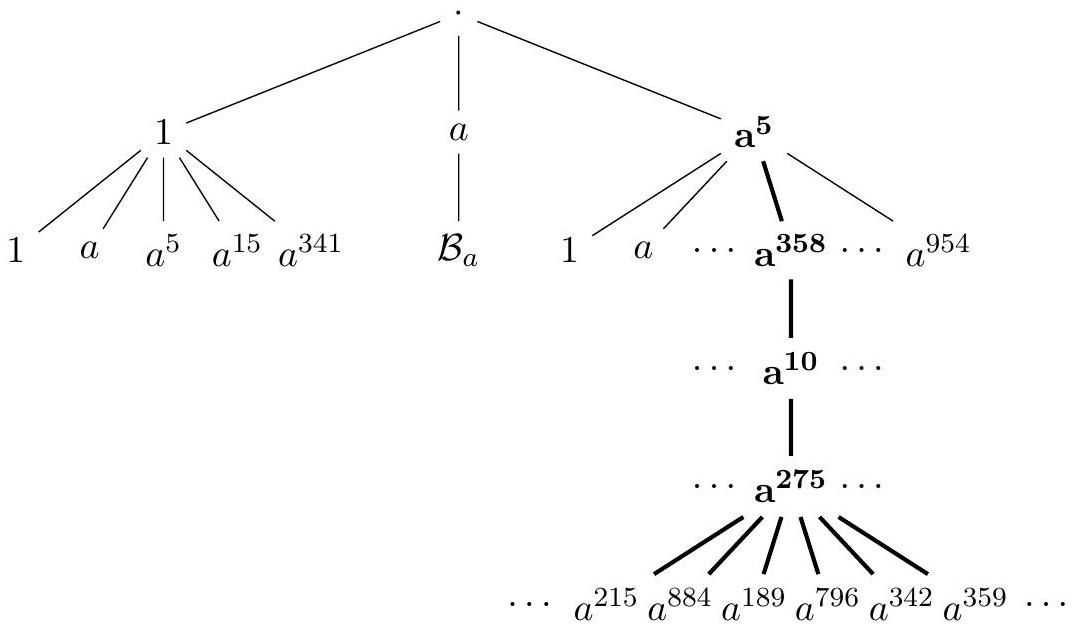
\includegraphics[alt={},max width=\textwidth]{63c8d736-eef8-427f-89a9-bfd33161edc8-24_629_1075_257_522}
\captionsetup{labelformat=empty}
\caption{Figure 7: Backward search with first 5 level of known APN function}
\end{center}
\end{figure}

\subsection*{5.4.1 Partial search for $\left\{a^{5},{ }^{358}, a^{10}, a^{275}, E\right\}$}
For $A=a^{5}, B=a^{358}, C=a^{10}, D=a^{275}, E=a^{215}$ brute-forcing last levels $F, G, H, I$ took 12 days to finish in 32 parallel processes. As we had 1023 candidates on each level, we applied an additional submatrix test for equivalent functions discovered in Section 4.5.1. Derivative matrices from Table 3 contain submatrices that are fast to check even for lower levels, helping to reduce the number of candidates for $F, G, H$.

Despite the large number of derivative matrices examined, only one function, given by (19), was found. The uniqueness of this result was unexpected, prompting us to explore one level above by examining other candidates of $E \in \mathcal{E}_{a^{5}, a^{358}, a^{10}, a^{275} \backslash a^{215}}$. There are 900 possible values for $E$ after the submatrix test, therefore it will take around 30 years to try each of the candidates. Therefore, we decided to randomly pick $E$ and check if there is another APN function inequivalent to 18 for this particular choice of branch. After trying 5 randomly chosen values for $E$, we did not find any APN functions and concluded the partial search, as summarized in Table 8.

\begin{table}[h]
\begin{center}
\begin{tabular}{|l|l|l|l|}
\hline
Value of $E$ & Number of cores & Time taken & APN functions \\
\hline
$a^{215}$ & 32 & 12 days & (19) \\
\hline
$a^{884}$ & 64 & 7 days & - \\
\hline
$a^{189}$ & 32 & 8 days & - \\
\hline
$a^{796}$ & 32 & 7,5 days & - \\
\hline
$a^{342}$ & 32 & 14 days & - \\
\hline
$a^{359}$ & 32 & 8 days & - \\
\hline
\end{tabular}
\captionsetup{labelformat=empty}
\caption{Table 8: Partial search for 5 levels fixed with the different $E$}
\end{center}
\end{table}

The same pattern, where the first levels determine only one APN function, was observed across all cases $(n, m)$. Therefore we hypothesize that the first four levels of this branch $\left\{a^{5},{ }^{358}, a^{10}, a^{275}\right\}$, define a single APN function.

\subsection*{5.4.2 Partial search for $\left\{a^{5},{ }^{358}, a^{421}, a^{349}, E\right\}$}
For the purposes of exploring other branches among $A=a^{5}, B=a^{358}$, we randomly selected $C=a^{421}$ and $D=a^{349}$. In this case, the partition remains efficient up to the sixth level. Moreover,\\
there are only four possible values for $E$ in $E s_{S u b}=\left\{a, a^{7}, a^{10}, a^{15}\right\}$, making it feasible to bruteforce all cases of $E$, unlike in the previous search. We perform the same search with the first five levels fixed as we did for 18, yet we take $A=a^{5}, B=a^{358} ; C=a^{421} ; D=a^{349}$, with $E \in\left\{a, a^{7}, a^{10}, a^{15}\right\}$, see Table 9.

\begin{table}[h]
\begin{center}
\begin{tabular}{|c|c|c|c|}
\hline
Value of $E$ & Number of cores & Time taken & APN functions \\
\hline
$a$ & 64 & 10 days & - \\
$a^{7}$ & 32 & 14 days & - \\
$a^{10}$ & 32 & 14 days & - \\
$a^{15}$ & 64 & 10 days & - \\
\hline
\end{tabular}
\captionsetup{labelformat=empty}
\caption{Table 9: Partial search for another 5 levels fixed}
\end{center}
\end{table}

\section*{6 Conclusion}
In this paper, we presented a series of significant improvements to the known QAM method for finding APN functions over $\mathbb{F}_{2^{n}}$ with coefficients in the subfield $\mathbb{F}_{2^{m}}$. First, we introduced orbit partitioning across several levels, showing how linear permutations can be used to reduce the search space on each level of the depth-first search. This allows us to effectively partition the finite field under the action of groups of linear permutations. Moreover, we propose an alternative method for cases where explicitly computing all permutations would have been impossible due to the lack of memory. We also developed a tree-based method to estimate the computation time of orbit partitioning. This helps us assess the feasibility of various cases, revealing that certain configurations, like $(n, m)=(10,2)$, are currently infeasible given computational constraints. Secondly, we improve the submatrix test that uses submatrices to terminate the check of the branches that never produce QAM. Applying the linear equivalence on the right, we could not only accelerate the submatrix test but also add additional conditions that helped us to terminate more unneeded branches. Finally, we accelerate the QAM check itself using Theorem 3, achieving up to a $50 \%$ increase in computational speed. By integrating all these enhancements into one algorithm, we completed a full classification for the cases $(n, m)=(8,2)$ and $(10,1)$, discovering a new APN function in $(8,2)$. Partial searches were also conducted for $(n, m)=(8,4)$, and $(10,2)$.

\section*{References}
[1] Simon Berg. The list of all found 27 inequivalent classes of quadratic functions over $\mathbb{F}_{2^{8}}$ with coefficients in $\mathbb{F}_{4}$. \href{https://github.com/Simon-Berg/thesis}{https://github.com/Simon-Berg/thesis}, 2023.\\[0pt]
[2] Wieb Bosma, John Cannon, and Catherine Playoust. The Magma algebra system. The user language, 1997.\\[0pt]
[3] Lilya Budaghyan, Claude Carlet, and Gregor Leander. Constructing new APN functions from known ones. Finite Fields and Their Applications, 15(2):150-159, 2009.\\[0pt]
[4] Lilya Budaghyan, Tor Helleseth, and Nikolay Kaleyski. A new family of APN quadrinomials. IEEE Transactions on Information Theory, 66(11):7081-7087, 2020.\\[0pt]
[5] Anne Canteaut, Alain Couvreur, and Léo Perrin. Recovering or testing extended-affine equivalence. Cryptology ePrint Archive, Paper 2021/225, 2021.\\[0pt]
[6] Claude Carlet. Boolean Functions for Cryptography and Coding Theory. Cambridge University Press, 2021.\\[0pt]
[7] Diana Davidova and Nikolay Kaleyski. Classification of all DO planar polynomials with prime field coefficients over $G F\left(3^{n}\right)$ for $n$ up to 7. Cryptology ePrint Archive, Paper 2022/1059, 2022. \href{https://eprint.iacr.org/2022/1059}{https://eprint.iacr.org/2022/1059}.\\[0pt]
[8] Yves Edel and Alexander Pott. A new almost perfect nonlinear function which is not quadratic. Cryptology ePrint Archive, Paper 2008/313, 2008.\\[0pt]
[9] Yves Edel and Alexander Pott. On the equivalence of nonlinear functions. In Enhancing cryptographic primitives with techniques from error correcting codes, pages 87-103. IOS Press, 2009.\\[0pt]
[10] Satoshi Yoshiara. Equivalences of quadratic APN functions. Journal of Algebraic Combinatorics, 35(3):461-475, 2012.\\[0pt]
[11] Yuyin Yu, Nikolay Kaleyski, Lilya Budaghyan, and Yongqiang Li. Classification of quadratic APN functions with coefficients in $\mathbb{F}_{2}$ for dimensions up to 9. Finite Fields and Their Applications, 68:101733, 2020.\\[0pt]
[12] Yuyin Yu, Jingchen Li, Nadiia Ichanska, and Nikolay Kaleyski. Construction of quadratic APN functions with coefficients in $\mathbb{F}_{2}$ in dimensions 10 and 11. Cryptology ePrint Archive, Paper 2024/1778, 2024.\\[0pt]
[13] Yuyin Yu and Leo Perrin. Constructing more quadratic APN functions with the QAM method. Cryptology ePrint Archive, Paper 2021/574, 2021.\\[0pt]
[14] Yuyin Yu, Mingsheng Wang, and Yongqiang Li. A matrix approach for constructing quadratic APN functions. Cryptology ePrint Archive, Paper 2013/007, 2013.\\[0pt]
[15] Yuyin Yu, Mingsheng Wang, and Yongqiang Li. A matrix approach for constructing quadratic APN functions. Designs, codes and cryptography, 73(2):587-600, 2014.

\section*{A Derivative matrices}
\section*{A. 1 Derivative matrix in the case $(n, m)=(8,4)$}
The structure of a derivative matrix for an arbitarary quadratic function over $\mathbb{F}_{2^{8}}$ with coefficients in the $\mathbb{F}_{2^{4}}$ is:

\[
M=\left(\begin{array}{cccccccc}
0 & A & B & C & D & E & F & G  \tag{20}\\
A & 0 & H & I & E^{2^{4}} & J & K & L \\
B & H & 0 & M & F^{2^{4}} & K^{2^{4}} & N & O \\
C & I & M & 0 & G^{2^{4}} & L^{2^{4}} & O^{2^{4}} & P \\
D & E^{2^{4}} & F^{2^{4}} & G^{2^{4}} & 0 & A^{2^{4}} & B^{2^{4}} & C^{2^{4}} \\
E & J & K^{2^{4}} & L^{2^{4}} & A^{2^{4}} & 0 & H^{2^{4}} & I^{2^{4}} \\
F & K & N & O^{2^{4}} & B^{2^{4}} & H^{2^{4}} & 0 & M^{2^{4}} \\
G & L & O & P & C^{2^{4}} & I^{2^{4}} & M^{2^{4}} & 0
\end{array}\right),
\]

where $A, B, C, E, F, G, H, I, K, L, M, O \in \mathbb{F}_{2^{8}}$, and $D, J, N, P \in \mathbb{F}_{2^{4}}$ that makes 16 variable.

\section*{A. 2 Derivative matrix in the case $(n, m)=(9,3)$}
The structure for derivative matrices for the quadratic functions over $\mathbb{F}_{2^{9}}$ with coefficients in the $\mathbb{F}_{2^{3}}$ is:

\[
M=\left(\begin{array}{ccccccccc}
0 & A & B & C & D & E & C^{2^{6}} & F & G  \tag{21}\\
A & 0 & H & F^{2^{3}} & I & J & D^{2^{6}} & I^{2^{6}} & K^{2^{6}} \\
B & H & 0 & G^{2^{3}} & K^{2^{3}} & L & E^{2^{6}} & J^{2^{6}} & L^{2^{6}} \\
C & F^{2^{3}} & G^{2^{3}} & 0 & A^{2^{3}} & B^{2^{3}} & C^{2^{3}} & D^{2^{3}} & E^{2^{3}} \\
D & I & K^{2^{3}} & A^{2^{3}} & 0 & H^{2^{3}} & F^{2^{6}} & I^{2^{3}} & J^{2^{3}} \\
E & J & L & B^{2^{3}} & H^{2^{3}} & 0 & G^{2^{6}} & K^{2^{6}} & L^{2^{3}} \\
C^{2^{6}} & D^{2^{6}} & E^{2^{6}} & C^{2^{3}} & F^{2^{6}} & G^{2^{6}} & 0 & A^{2^{6}} & B^{2^{6}} \\
F & I^{2^{6}} & J^{2^{6}} & D^{2^{3}} & I^{2^{3}} & K^{2^{6}} & A^{2^{6}} & 0 & H^{2^{6}} \\
G & K^{2^{6}} & L^{2^{6}} & E^{2^{3}} & J^{2^{3}} & L^{2^{3}} & B^{2^{6}} & H^{2^{6}} & 0
\end{array}\right),
\]

where $A, B, C, D, E, F, G, H, I, J, K, L \in \mathbb{F}_{2^{9}}$.

\section*{A. 3 Derivative matrix in the case $(n, m)=(10,1)$}
The structure for a derivative matrix for the quadratic functions $F$ over $\mathbb{F}_{2^{1} 0}$ with coefficients in the $\mathbb{F}_{2}$ is:

\[
M=\left(\begin{array}{cccccccccc}
0 & A & B & C & D & E & D^{2^{6}} & C^{2^{7}} & B^{2^{8}} & A^{2^{9}}  \tag{22}\\
A & 0 & A^{2} & B^{2} & C^{2} & D^{2} & E^{2} & D^{2^{7}} & C^{2^{8}} & B^{2^{9}} \\
B & A^{2} & 0 & A^{2^{2}} & B^{2^{2}} & C^{2^{2}} & D^{2^{2}} & E^{2^{2}} & D^{2^{8}} & C^{2^{9}} \\
C & B^{2} & A^{2^{2}} & 0 & A^{2^{3}} & B^{2^{3}} & C^{2^{3}} & D^{2^{3}} & E^{2^{8}} & D^{2^{9}} \\
D & C^{2} & B^{2^{2}} & A^{2^{3}} & 0 & A^{2^{4}} & B^{2^{4}} & C^{2^{4}} & D^{2^{4}} & E^{2^{4}} \\
E & D^{2} & C^{2^{2}} & B^{2^{3}} & A^{2^{4}} & 0 & A^{2^{5}} & B^{2^{5}} & C^{2^{5}} & D^{2^{5}} \\
D^{2^{6}} & E^{2^{2}} & D^{2^{2}} & C^{2^{3}} & B^{2^{4}} & A^{2^{5}} & 0 & A^{2^{6}} & B^{2^{6}} & C^{2^{6}} \\
C^{2^{7}} & D^{2^{7}} & E^{2^{3}} & D^{2^{4}} & C^{2^{4}} & B^{2^{5}} & A^{2^{6}} & 0 & A^{2^{7}} & B^{2^{7}} \\
B^{2^{8}} & C^{2^{8}} & D^{2^{8}} & E^{2^{4}} & D^{2^{4}} & C^{2^{5}} & B^{2^{6}} & A^{2^{7}} & 0 & A^{2^{8}} \\
A^{2^{9}} & B^{2^{9}} & C^{2^{9}} & D^{2^{9}} & E^{2^{5}} & D^{2^{5}} & C^{2^{6}} & B^{2^{7}} & A^{2^{8}} & 0
\end{array}\right) .
\]

\section*{A. 4 Derivative matrix in the case $(n, m)=(10,2)$}
The structure for a derivative matrix for the quadratic functions over $\mathbb{F}_{2^{1} 0}$ with coefficients in the $\mathbb{F}_{2^{2}}$ is:

\[
M=\left(\begin{array}{cccccccccc}
0 & A & B & C & D & E & D^{2^{6}} & F & B^{2^{8}} & G  \tag{23}\\
A & 0 & G^{2^{2}} & H & F^{2^{4}} & I & E^{2^{6}} & I^{2^{6}} & C^{2^{8}} & H^{2^{8}} \\
B & G^{2^{2}} & 0 & A^{2^{2}} & B^{2^{2}} & C^{2^{2}} & D^{2^{2}} & E^{2^{2}} & D^{2^{8}} & F^{2^{2}} \\
C & H & A^{2^{2}} & 0 & G^{2^{4}} & H^{2^{2}} & F^{2^{6}} & I^{2^{2}} & E^{2^{8}} & I^{2^{8}} \\
D & F^{2^{4}} & B^{2^{2}} & G^{2^{4}} & 0 & A^{2^{4}} & B^{2^{4}} & C^{2^{4}} & D^{2^{4}} & E^{2^{4}} \\
E & I & C^{2^{2}} & H^{2^{2}} & A^{2^{4}} & 0 & G^{2^{6}} & H^{2^{4}} & F^{2^{8}} & I^{2^{4}} \\
D^{2^{6}} & E^{2^{6}} & D^{2^{2}} & F^{2^{6}} & B^{2^{4}} & G^{2^{6}} & 0 & A^{2^{6}} & B^{2^{6}} & C^{2^{6}} \\
F & I^{2^{6}} & E^{2^{2}} & I^{2^{2}} & C^{2^{4}} & H^{2^{4}} & A^{2^{6}} & 0 & G^{2^{8}} & H^{2^{6}} \\
B^{2^{8}} & C^{2^{8}} & D^{2^{8}} & E^{2^{8}} & D^{2^{4}} & F^{2^{8}} & B^{2^{6}} & G^{2^{8}} & 0 & A^{2^{8}} \\
G & H^{2^{8}} & F^{2^{2}} & I^{2^{8}} & E^{2^{4}} & I^{2^{4}} & C^{2^{6}} & H^{2^{6}} & A^{2^{8}} & 0
\end{array}\right),
\]

where $A, B, C, D, E, F, G, H, I \in \mathbb{F}_{2^{n}}$.\\
If $M_{F}$ represent a derivative matrix (23) of the function $F$, then the derivative matrix of the equivalent function $F^{\prime}=F \circ \alpha x^{2}, \alpha \in \mathbb{F}_{4}$ will look like:

\[
M^{(1)}=\left(\begin{array}{cccccccccc}
0 & G^{2^{2}} & H & F^{2^{4}} & I & E^{2^{6}} & I^{2^{6}} & C^{2^{8}} & H^{2^{8}} & A  \tag{24}\\
G^{2^{2}} & 0 & A^{2^{2}} & B^{2^{2}} & C^{2^{2}} & D^{2^{2}} & E^{2^{2}} & D^{2^{8}} & F^{2^{2}} & B \\
H & A^{2^{2}} & 0 & G^{2^{4}} & H^{2^{2}} & F^{2^{6}} & I^{2^{2}} & E^{2^{8}} & I^{2^{8}} & C \\
F^{2^{4}} & B^{2^{2}} & G^{2^{4}} & 0 & A^{2^{4}} & B^{2^{4}} & C^{2^{4}} & D^{2^{4}} & E^{2^{4}} & D \\
I & C^{2^{2}} & H^{2^{2}} & A^{2^{4}} & 0 & G^{2^{6}} & H^{2^{4}} & F^{2^{8}} & I^{2^{4}} & E \\
E^{2^{6}} & D^{2} & F^{2^{6}} & B^{2^{4}} & G^{2^{6}} & 0 & A^{2^{6}} & B^{2^{6}} & C^{2^{6}} & D^{2^{6}} \\
I^{2^{6}} & E^{2^{2}} & I^{2^{2}} & C^{2^{4}} & H^{2^{4}} & A^{2^{6}} & 0 & G^{2^{8}} & H^{2^{6}} & F \\
C^{2^{8}} & D^{2^{8}} & E^{2^{8}} & D^{2^{4}} & F^{2^{8}} & B^{2^{6}} & G^{2^{8}} & 0 & A^{2^{8}} & B^{2^{8}} \\
H^{2^{8}} & F^{2^{2}} & I^{2^{8}} & E^{2^{4}} & I^{2^{4}} & C^{2^{6}} & H^{2^{6}} & A^{2^{8}} & 0 & G \\
A & B & C & D & E & D^{2^{6}} & F & B^{2^{8}} & G & 0
\end{array}\right) .
\]

Take the APN function $F(x)=x^{288}+a^{682} x^{96}+a^{341} x^{9}+x^{3}(18)$.\\
Fixing the normal element $a^{486}$ for a basis we get the derivative matrix $M_{F}$ of the function $F$ :

\[
M_{F}=\left[\begin{array}{cccccccccc}
0 & a^{719} & a^{851} & a^{146} & a^{84} & a^{708} & a^{261} & a^{709} & a^{980} & a^{785}  \tag{25}\\
a^{719} & 0 & a^{71} & a^{117} & a^{91} & a^{259} & a^{300} & a^{208} & a^{548} & a^{285} \\
a^{851} & a^{71} & 0 & a^{830} & a^{335} & a^{584} & a^{336} & a^{786} & a^{21} & a^{790} \\
a^{146} & a^{117} & a^{830} & 0 & a^{284} & a^{468} & a^{364} & a^{13} & a^{177} & a^{832} \\
a^{84} & a^{91} & a^{335} & a^{284} & 0 & a^{251} & a^{317} & a^{290} & a^{321} & a^{75} \\
a^{708} & a^{259} & a^{584} & a^{468} & a^{251} & 0 & a^{113} & a^{849} & a^{433} & a^{52} \\
a^{261} & a^{300} & a^{336} & a^{364} & a^{317} & a^{113} & 0 & a^{1004} & a^{245} & a^{137} \\
a^{709} & a^{208} & a^{786} & a^{13} & a^{290} & a^{849} & a^{1004} & 0 & a^{452} & a^{327} \\
a^{980} & a^{548} & a^{21} & a^{177} & a^{321} & a^{433} & a^{245} & a^{452} & 0 & a^{947} \\
a^{785} & a^{285} & a^{790} & a^{832} & a^{75} & a^{52} & a^{137} & a^{327} & a^{947} & 0
\end{array}\right] .
\]

For the equivalent to (18) functions $F^{\prime}(19)$ which is:

$$
\begin{array}{r}
F^{\prime}=l(F)=x^{768}+a^{682} x^{516}+a^{341} x^{513}+a^{682} x^{384}+x^{258}+a^{341} x^{192}+x^{144}+x^{129}+ \\
+a^{682} x^{72}+a^{682} x^{48}+a^{341} x^{36}+a^{682} x^{24}+x^{12}+x^{6}
\end{array}
$$

the derivative matrix $M_{F^{\prime}}$ for the same basis is:

\[
M_{F^{\prime}}=\left[\begin{array}{cccccccccc}
0 & a^{5} & a^{358} & a^{10} & a^{275} & a^{215} & a^{209} & a^{659} & a^{601} & a^{651}  \tag{26}\\
a^{5} & 0 & a^{558} & a^{225} & a^{314} & a^{11} & a^{461} & a^{704} & a^{514} & a^{312} \\
a^{358} & a^{558} & 0 & a^{20} & a^{409} & a^{40} & a^{77} & a^{860} & a^{836} & a^{590} \\
a^{10} & a^{225} & a^{20} & 0 & a^{186} & a^{900} & a^{233} & a^{44} & a^{821} & a^{770} \\
a^{275} & a^{314} & a^{409} & a^{186} & 0 & a^{80} & a^{613} & a^{160} & a^{308} & a^{371} \\
a^{215} & a^{11} & a^{40} & a^{900} & a^{80} & 0 & a^{744} & a^{531} & a^{932} & a^{176} \\
a^{209} & a^{461} & a^{77} & a^{233} & a^{613} & a^{744} & 0 & a^{320} & a^{406} & a^{640} \\
a^{659} & a^{704} & a^{860} & a^{44} & a^{160} & a^{531} & a^{320} & 0 & a^{930} & a^{78} \\
a^{601} & a^{514} & a^{836} & a^{821} & a^{308} & a^{932} & a^{406} & a^{930} & 0 & a^{257} \\
a^{651} & a^{312} & a^{590} & a^{770} & a^{371} & a^{176} & a^{640} & a^{78} & a^{257} & 0
\end{array}\right] .
\]

\section*{B Tables for the classification of the quadratic functions over $\mathbb{F}_{2^{8}}$ with coefficients in $\mathbb{F}_{4}$}
\begin{table}[h]
\begin{center}
\begin{tabular}{|l|l|}
\hline
Index & Representative functions \\
\hline
1 & $x^{192}+x^{96}+x^{72}+x^{33}+x^{3}$ \\
\hline
2 & $a^{170} x^{144}+a^{85} x^{72}+a^{85} x^{48}+a^{85} x^{24}+a^{85} x^{12}+x^{9}+x^{3}$ \\
\hline
3 & $x^{72}+x^{66}+x^{48}+x^{36}+a^{170} x^{33}+x^{18}+x^{9}+a^{170} x^{6}+a^{85} x^{3}$ \\
\hline
4 & $a^{170} x^{192}+a^{85} x^{144}+a^{85} x^{132}+a^{170} x^{66}+a^{85} x^{48}+x^{33}+x^{24}+a^{170} x^{18}+a^{85} x^{6}+x^{3}$ \\
\hline
5 & $a^{170} x^{144}+a^{85} x^{132}+x^{96}+a^{170} x^{72}+a^{170} x^{36}+x^{33}+a^{85} x^{24}+x^{12}+x^{3}$ \\
\hline
6 & $a^{170} x^{192}+a^{85} x^{132}+a^{170} x^{66}+a^{170} x^{24}+a^{170} x^{18}+a^{170} x^{12}+x^{6}+x^{3}$ \\
\hline
7 & $a^{85} x^{192}+a^{170} x^{144}+a^{170} x^{96}+a^{85} x^{72}+a^{170} x^{66}+x^{36}+x^{12}+x^{3}$ \\
\hline
8 & $a^{85} x^{144}+a^{170} x^{129}+a^{170} x^{72}+a^{170} x^{18}+x^{12}+a^{85} x^{9}+x^{3}$ \\
\hline
9 & $a^{170} x^{132}+a^{170} x^{96}+a^{85} x^{72}+a^{85} x^{66}+x^{48}+a^{170} x^{18}+x^{6}+x^{3}$ \\
\hline
10 & $a^{85} x^{96}+a^{85} x^{72}+a^{170} x^{24}+x^{18}+a^{85} x^{12}+a^{85} x^{9}+x^{6}+x^{3}$ \\
\hline
11 & $x^{132}+a^{85} x^{96}+a^{170} x^{72}+a^{85} x^{48}+x^{33}+x^{24}+a^{170} x^{12}+a^{170} x^{6}+x^{3}$ \\
\hline
12 & $a^{170} x^{144}+a^{85} x^{132}+x^{72}+a^{170} x^{48}+a^{170} x^{24}+x^{18}+a^{170} x^{12}+x^{3}$ \\
\hline
13 & $a^{85} x^{144}+a^{85} x^{66}+a^{170} x^{65}+a^{85} x^{48}+x^{36}+a^{170} x^{33}+a^{170} x^{20}+a^{170} x^{18}+x^{9}+x^{3}$ \\
\hline
14 & \multirow{2}{*}{\begin{tabular}{l}
$a^{170} x^{160}+a^{85} x^{144}+a^{85} x^{132}+a^{85} x^{96}+a^{85} x^{80}+a^{85} x^{68}+a^{85} x^{66}+a^{85} x^{48}+x^{18}+a^{170} x^{5}+x^{3}$ \\
$a^{85} x^{160}+a^{85} x^{136}+a^{85} x^{96}+a^{170} x^{40}+a^{85} x^{36}+a^{85} x^{34}+x^{20}+a^{85} x^{17}+x^{12}+x^{9}+x^{3}$ \\
\end{tabular}} \\
\hline
15 &  \\
\hline
16 & $x^{160}+a^{170} x^{144}+a^{85} x^{129}+a^{170} x^{96}+a^{170} x^{68}+a^{170} x^{40}+x^{20}+a^{85} x^{18}+a^{170} x^{12}+x^{9}+x^{3}$ \\
\hline
17 & $a^{85} x^{192}+a^{85} x^{160}+a^{85} x^{132}+a^{170} x^{72}+x^{48}+x^{40}+x^{34}+x^{33}+x^{18}+a^{170} x^{10}+x^{3}$ \\
\hline
18 & $a^{85} x^{136}+a^{85} x^{132}+x^{96}+a^{170} x^{72}+a^{85} x^{68}+a^{85} x^{66}+x^{48}+x^{33}+a^{85} x^{17}+x^{3}$ \\
\hline
19 & $a^{170} x^{192}+a^{85} x^{132}+x^{129}+a^{85} x^{80}+a^{85} x^{68}+x^{48}+x^{24}+x^{20}+x^{10}+a^{85} x^{5}+x^{3}$ \\
\hline
20 & $a^{170} x^{144}+a^{170} x^{136}+x^{132}+a^{170} x^{80}+a^{85} x^{66}+a^{170} x^{65}+a^{170} x^{34}+a^{170} x^{33}+x^{24}+a^{170} x^{18}+x^{9}+a^{85} x^{6}+x^{3}$ \\
\hline
21 & $a^{170} x^{144}+x^{136}+x^{129}+a^{85} x^{68}+a^{85} x^{66}+x^{65}+a^{170} x^{48}+a^{170} x^{40}+a^{85} x^{36}+x^{33}+a^{170} x^{17}+a^{170} x^{12}+x^{3}$ \\
\hline
22 & $x^{192}+a^{85} x^{144}+a^{85} x^{68}+a^{170} x^{65}+a^{85} x^{48}+a^{170} x^{40}+a^{85} x^{24}+a^{170} x^{20}+a^{170} x^{18}+a^{85} x^{17}+a^{170} x^{10}+x^{3}$ \\
\hline
23 & \multirow{2}{*}{\begin{tabular}{l}
$a^{85} x^{192}+a^{85} x^{144}+x^{36}+x^{33}+a^{170} x^{24}+a^{170} x^{18}+x^{12}+x^{6}+x^{3}$ \\
$x^{192}+x^{160}+a^{85} x^{130}+a^{85} x^{96}+a^{170} x^{72}+x^{66}+a^{170} x^{48}+x^{40}+a^{85} x^{33}+a^{85} x^{18}+x^{5}+x^{3}$ \\
\end{tabular}} \\
\hline
24 &  \\
\hline
25 & $a^{85} x^{192}+a^{170} x^{160}+x^{144}+x^{130}+a^{170} x^{129}+x^{65}+a^{170} x^{40}+a^{85} x^{34}+a^{85} x^{24}+a^{170} x^{20}+a^{170} x^{18}+a^{170} x^{9}+x^{3}$ \\
\hline
26 & \multirow{2}{*}{$a^{85} x^{129}+a^{85} x^{96}+x^{72}+a^{85} x^{66}+x^{12}+a^{170} x^{9}+x^{6}+x^{3}$
$a^{170} x^{160}+a^{170} x^{136}+a^{85} x^{132}+a^{170} x^{129}+a^{85} x^{68}+a^{170} x^{40}+x^{33}+a^{85} x^{24}+a^{85} x^{9}+a^{170} x^{6}+x^{3}$} \\
\hline
27 &  \\
\hline
\end{tabular}
\captionsetup{labelformat=empty}
\caption{Table 10: Representatives up to CCZ-equivalence of all quadratic APN functions over $\mathbb{F}_{2^{8}}$ with coefficients in $\mathbb{F}_{2^{2}}$, with the new found function in bold}
\end{center}
\end{table}

\begin{table}[h]
\begin{center}
\begin{tabular}{|l|l|}
\hline
Index & ODDS \\
\hline
1 & $\left[0^{35700}, 2^{26520}, 4^{3060}\right]$ \\
\hline
2 & $\left[0^{36420}, 2^{25080}, 4^{3780}\right]$ \\
\hline
3 & $\left[0^{37872}, 2^{22788}, 4^{4068}, 6^{492}, 8^{60}\right]$ \\
\hline
4 & $\left[0^{37980}, 2^{22272}, 4^{4716}, 6^{312}\right]$ \\
\hline
5 & $\left[0^{38004}, 2^{22614}, 4^{4008}, 6^{630}, 10^{24}\right]$ \\
\hline
6 & $\left[0^{38040}, 2^{22461}, 4^{4218}, 6^{513}, 8^{36}, 10^{12}\right]$ \\
\hline
7 & $\left[0^{38160}, 2^{22104}, 4^{4536}, 6^{456}, 8^{24}\right]$ \\
\hline
8 & $\left[0^{38160}, 2^{22164}, 4^{4428}, 6^{492}, 8^{36}\right]$ \\
\hline
9 & $\left[0^{38184}, 2^{22179}, 4^{4338}, 6^{531}, 8^{48}\right]$ \\
\hline
10 & $\left[0^{38196}, 2^{22008}, 4^{4608}, 6^{456}, 8^{12}\right]$ \\
\hline
11 & $\left[0^{38256}, 2^{22116}, 4^{4230}, 6^{648}, 8^{30}\right]$ \\
\hline
12 & $\left[0^{38592}, 2^{21426}, 4^{4590}, 6^{654}, 8^{18}\right]$ \\
\hline
13 & $\left[0^{38844}, 2^{20974}, 4^{4764}, 6^{654}, 8^{44}\right]$ \\
\hline
14 & $\left[0^{38880}, 2^{21165}, 4^{4230}, 6^{1005}\right]$ \\
\hline
15 & $\left[0^{39174}, 2^{20513}, 4^{4756}, 6^{749}, 8^{76}, 10^{8}, 12^{4}\right]$ \\
\hline
16 & $\left[0^{39290}, 2^{20399}, 4^{4686}, 6^{774}, 8^{112}, 10^{15}, 12^{4}\right]$ \\
\hline
17 & $\left[0^{39408}, 2^{20072}, 4^{4922}, 6^{798}, 8^{70}, 10^{10}\right]$ \\
\hline
18 & $\left[0^{39408}, 2^{20218}, 4^{4692}, 6^{838}, 8^{104}, 10^{12}, 12^{8}\right]$ \\
\hline
19 & $\left[0^{39444}, 2^{20042}, 4^{4912}, 6^{762}, 8^{112}, 10^{8}\right]$ \\
\hline
20 & $\left[0^{39446}, 2^{20067}, 4^{4896}, 6^{718}, 8^{138}, 10^{15}\right]$ \\
\hline
21 & $\left[0^{39504}, 2^{20127}, 4^{4674}, 6^{801}, 8^{138}, 10^{27}, 16^{6}, 18^{3}\right]$ \\
\hline
22 & $\left[0^{39544}, 2^{19996}, 4^{4752}, 6^{841}, 8^{130}, 10^{12}, 12^{2}, 14^{1}, 18^{2}\right]$ \\
\hline
23 & $\left[0^{39600}, 2^{19680}, 4^{5220}, 6^{600}, 8^{180}\right]$ \\
\hline
24 & $\left[0^{39692}, 2^{19752}, 4^{4756}, 6^{978}, 8^{72}, 10^{26}, 12^{4}\right]$ \\
\hline
25 & $\left[0^{39750}, 2^{19641}, 4^{4876}, 6^{845}, 8^{136}, 10^{29}, 14^{2}, 18^{1}\right]$ \\
\hline
26 & $\left[0^{39780}, 2^{21930}, 6^{3570}\right]$ \\
\hline
27 & $\left[0^{39840}, 2^{19707}, 4^{4644}, 6^{900}, 8^{120}, 10^{9}, 14^{60}\right]$ \\
\hline
\end{tabular}
\captionsetup{labelformat=empty}
\caption{Table 11: The ortho-derivative differential spectrum of all quadratic APN functions over $\mathbb{F}_{2^{8}}$ with coefficients in $\mathbb{F}_{2^{2}}$, with the ODDS of the new found function in bold}
\end{center}
\end{table}


\end{document}